% ---------------------------------------------------------------------
%                        LATEX TEMPLATE FOR 
%                    BACHELOR'S / MASTER'S / Ph.D 
%                     THESIS AT LUND UNIVERSITY
% ---------------------------------------------------------------------

%%% Compiling with XeLaTeX -> LU fonts: Adobe Garamond Pro and Frutiger %%%

%%% Compiling with PDFLaTeX -> Latin Modern fonts %%%

\documentclass[a4, nocrop, rm, english]{luthesis}

% LUTHESIS CLASS OPTIONS
%
% thesis      - Master's or Ph.D thesis, 17x24 cm
% a4          - Bachelor's thesis, A4 format 21x29.7 cm
% rm          - Roman typeface
% sf          - Sans serif typeface
% crop        - Crop marks (cross) 17x24 cm (+3 mm on all four corners) centered on an A4
% nocrop      - No crop marks, respect size 
% nomathskip  - The distances of the equations are not modified 
% swedish     - The publication is written in Swedish
% english     - The publication is written in English

% ---------------------------------------------------------------------
% Custom settings and bibliography file 'references.bib'

\input{preamble}

\bibliography{references}

% ---------------------------------------------------------------------
% Folders for graphics

\graphicspath{
	{../figures/}
	{../logos/}
	{./figures/}
	{./logos/}
}

% ---------------------------------------------------------------------
% Title and author are not really necessary since a pdf will be used as a cover later

\title{
	Thesis template example title made with \LaTeX\ \\[3ex]
	\mdseries\large	July 2020
}

\author{
	Francisco García Atienza
}

% ---------------------------------------------------------------------
% Making index and glossary files

%\makeindex

\makeglossaries
\input{chapters/glossary}

% ---------------------------------------------------------------------
% ---------------------------------------------------------------------

\begin{document}
	
	% -------------------------------------------------------
	% Redefining cross references names according to language 
	% or personal preferences, Bibliography->References, Appendix->Paper, etc.
	
	\input{cross_references}
	
	% -------------------------------------------------------
	
	\frontmatter
	
	% -------------------------------------------------------
	% FRONT COVER 
	
	\includepdf{covers/frontbachelorcover} 
	%\includepdf{covers/blank}
	%\maketitle
	
	% TITLE / COPYRIGHT PAGE 
	%\includepdf[pages=-]{covers/title} 
	%%%\includepdf[pages=-]{covers/copyright_page}
	%\includepdf{logos/phdtitle}
	%\cleardoublepage
	% Start of page numbering
	\setcounter{page}{1}
	
	% Special headers for abstract,ack and contents in A4 format
	\ifAfour
	\pagestyle{preamb}
	\else
	
	\fi
	
	% -------------------------------------------------------
	% ABSTRACT
	
	\cleardoublepage
	\phantomsection
	\addcontentsline{toc}{chapter}{\abstractname}
	
	% ---------------------------------------------------------------------
% ---------------------------------------------------------------------
% ---------------------------------------------------------------------

\chapter*{\abstractname}
\markboth{Abstract}{}
% ---------------------------------------------------------------------
% ---------------------------------------------------------------------
% ---------------------------------------------------------------------
Static methods based on discrete snapshots or timeslices for measuring node interaction in networks that change over time do not fully capture the dynamical nature of network evolution. The present study provides a novel continuous-time approach to network centrality, a fundamental concept in network analysis.

To address this issue, a dynamical system model driven by network's continuous-time adjacency matrix is derived from a continuous version of Katz centrality, one of the most widely used centrality measures. Using this approach, numerical experiments are conducted on various networks, synthetic and real, showing that this continuous-time framework performs better than traditional static or aggregate measures and that it is able to capture dynamic effects of communication between nodes or even changes in the network structure over time.

The most significant conclusions of this work are that the new ODE-based framework offers major improvements in accuracy and efficiency over static methods for network simulations. By using advanced numerical ODE solvers, time discretization is performed automatically "under the hood" in an optimal and efficient manner, allowing the system to adapt to sudden and significant changes in network behavior. The ODE system’s property of downweighting information over time also enables real-time monitoring of centrality rankings without the need to store or account for all previous node interaction history. Moreover, it is shown why tracking good receivers of information in a dynamic network is cheaper than tracking good broadcasters from a computational cost perspective. 

Overall, this dynamical systems approach to network centrality can lead to new insights into the behavior of complex networks and has implications for a wide range of applications, from social networks to fluid mechanics, where network dynamics play a crucial role.


% ---------------------------------------------------------------------

	
	% -------------------------------------------------------
	% LIST OF PAPERS
	
	%\cleardoublepage
	%\phantomsection
	%\addcontentsline{toc}{chapter}{List of Papers}
	
	%\input{chapters/papers}
	
	% ------------------------------------------------------- 
	% Glossary
	
	%\cleardoublepage
	%\phantomsection
	%\addcontentsline{toc}{chapter}{Glossary}
	
	%\printglossary
	% Add the rest of entries if desired...
	%\glsaddallunused
	
	% -------------------------------------------------------
	% ACKNOWLEDGEMENTS, DEDICATION AND FAMOUS QUOTE
	
	%%%\cleardoublepage
	%%%\phantomsection
	%%%\addcontentsline{toc}{chapter}{Acknowledgements}
	%\addcontentsline{toc}{chapter}{Tack}
	
        %%%% ---------------------------------------------------------------------
% ---------------------------------------------------------------------
% ---------------------------------------------------------------------

\chapter*{Acknowledgements}
%\chapter*{Tack}

%\begin{quote}
%	\begin{flushright}
%		\textit{Life is like riding a bicycle. To keep your balance, you must keep moving.} \\
		
%		-- \textbf{Albert Einstein} --
%	\end{flushright}
%\end{quote}

% ---------------------------------------------------------------------
% ---------------------------------------------------------------------
% ---------------------------------------------------------------------

With this Bachelor's degree project, a fascinating journey ends and a new one begins. I would like to thank all the teachers and classmates I have had throughout these three years. From each and every one of them I have learned, and am still learning, to be a better mathematician.

Special thanks to my examiner Philipp Birken, for presenting me with a very interesting thesis subject, and to my supervisor, Viktor Linders, for his invaluable advice and guidance from the beginning of this project. 

Thanks to my family for their unconditional love.

Finally, and above all, this thesis work is dedicated to my lovely husband, Alfredo, who has been a constant source of love and support. Thanks for believing in me more than myself and teaching me that with humility, work and effort, dreams can be achieved in life.

\addvspace{1.3cm}

\textit{Lund, May 2023} \hfill \textit{Francisco García Atienza}


%\vspace*{2cm}






% ---------------------------------------------------------------------


	
	%\cleardoublepage
	%\input{chapters/dedication}
	%\cleardoublepage
	%\input{chapters/quote}
	
	% -------------------------------------------------------
	% TABLE OF CONTENTS
	
	\cleardoublepage
	\phantomsection
	\addcontentsline{toc}{chapter}{\contentsname}
	
	\ifAfour %%%% ONLY for A4 %%%%
	\tableofcontents
	\cleardoublepage
	\pagestyle{myfancy}
	\else
	\tableofcontents
	\fi
	
	% -------------------------------------------------------
	% MAINMATTER 
	
	\mainmatter
	
	% -------------------------------------------------------
	% -------------------------------------------------------
	% -------------------------------------------------------
	% CHAPTERS
	
	% ---------------------------------------------------------------------
% ---------------------------------------------------------------------
% ---------------------------------------------------------------------

\chapter[Introduction]{Introduction}
\label{chap:intro}

Networks are fundamental in many fields of science as they provide a powerful way to model complex systems and relationships between entities at different scales. By representing entities as nodes and connections between them as edges, networks can help researchers understand how information, energy, materials, and other resources flow through a system, identify patterns and structures within the data, and make predictions about system behavior. Many real life problems can be modeled as graphs or discretized as networks and that is why they are widely used in many fields such as physics, biology, sociology, statistics, or computer science amomg others. Network analysis in all these areas have led to significant advances in our understanding of the world around us \cite{albert2002statistical, katz1953new}, \cite[Part I]{newman2018networks}.

\section{Mathematical notation}
\label{sec:graph}
This section introduces a brief review of the definitions and notation pertaining to graphs, as well as some of their matrix representations, that will be used later in this study.

A network in the mathematical literature is, in its simplest form, a collection of interconnected nodes or vertices that represent entities, and the connections or edges between these nodes that represent relationships or interactions between the entities \cite{arrigo2022dynamic}.

\begin{definition}
    A weighted network, or graph, is an ordered triple of sets $G = (V, E, \mathcal{W})$, where $V$ is the set of nodes, $E\subset V\times V$ is the set of edges among the nodes and $\mathcal{W}$ is a map that assigns to each edge a weight or cost, usually a positive real number. When all these weights are given the same relevance or weight (by convention, $\omega=1$), then the graph, represented only by $G = (V, E)$, is called unweighted.
\end{definition}

The following two definitions that are central for this work are the concept of \textit{walk} and the \textit{adjacency matrix} of a graph.  

\begin{definition}
    A walk of length $w$ is a sequence of $w$ edges $(e_1, e_2, \dots, e_w)$ such that the target of $e_\ell$ coincides with the source of $e_{\ell+1}$ for all $\ell=1, 2, ..., w−1$.
\end{definition}
  
\begin{definition}
	Let $G =(V, E, \mathcal{W})$ be a weighted graph with $N$ nodes. Its adjacency matrix $\mathbf{A}\in\mathbb{R}^{N\times N}$ is entry-wise defined as
 
 \begin{equation}
  A_{ij} =
    \begin{cases}
      \sum_{e_{ij}}\omega_{ij} & \text{if there is an edge $e_{ij}$ between nodes $i$ and $j$ with cost $\omega_{ij}$},\\
      0 & \text{otherwise},
    \end{cases}       
\end{equation}
for all $i, j = 1,2,\dots, N$.
\end{definition}

Unless otherwise stated, all graphs analyzed in this study will be considered \textit{simple networks}.

\begin{definition}
    A simple network is a type of network where each edge connects only two distinct nodes, i.e., there are no self-loops or multiple edges between the same pair of nodes. 
\end{definition}
As a particular case, the adjacency matrix for simple unweighted graphs will have all their non-zero entries set to $A_{ij}=1$, indicating a link between nodes $i$ and $j$.

Additionally, graphs are usually represented visually using a diagram (e.g., Fig. \ref{fig:graphsv}), where nodes are represented as points and edges are represented as lines connecting the points. The direction of the edges allows us to divide graphs into \textit{directed} and \textit{undirected}. As a consequence of this, undirected graphs are represented by symmetric adjacency matrices, i.e., $A_{ij}=A_{ji}$ and, on the contrary, directed graphs by asymmetric matrices, $A_{ij}\ne A_{ji}$. The presence of loops, i.e., edges connecting a node to itself can also be indicated in this visual representation, $A_{ii} = 1$, in terms of the adjacency matrix.

\begin{figure}[h]\centering
	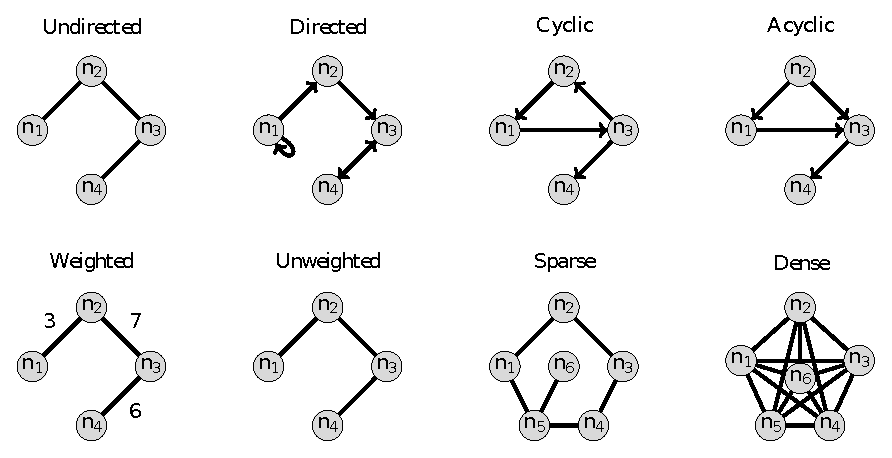
\includegraphics[width=0.75\textwidth]{graphsv}
	\caption{Examples of different network properties.}
	\label{fig:graphsv}
	\bigskip
\end{figure}

It is also worth mentioning other relevant network properties of graph theory for this work as:

\begin{itemize}
  \item \textit{Cyclic/Acyclic networks}: Cyclic networks are networks where there is at least one path from a node to itself. In other words, they contain cycles or loops. Examples of cyclic networks include recurrent neural networks (RNNs) and feedback loops in control systems. On the other hand, acyclic networks are networks that do not contain any cycles so there is no path from any node back to itself. Examples of these networks are directed acyclic graphs (DAGs) as directed binary trees.
  \item \textit{Sparse/Dense networks}: respectively, a sparse/dense network is a type of network where the number of edges (or connections) between nodes is/is not much smaller than the maximum possible number of edges in the network, resulting in a relatively low/high density of connections. Although there is a widespread agreement that most empirical networks are sparse, there is no formal definition of sparsity for any finite network, being the notion of "much smaller" purely colloquial.
  \item \textit{Static/Dynamic networks}: A static network is a network that does not change over time. The relationships and connections between nodes are fixed and remain constant. On the contrary, a dynamic network is a network that changes over time. The relationships and connections between nodes can evolve and alter, resulting in a continually changing network structure.
\end{itemize}

Linear algebra will play a significant role in network analysis as graphs are represented by matrices. The analysis of networks often involves solving linear systems, determining eigenvalues and eigenvectors, and evaluating matrix functions. Moreover, the examination of dynamic processes on graphs will create systems of differential equations based on their structure. The behavior of the solution over time is expected to be highly impacted by the graph's structure (network topology), which is reflected in the spectral properties of the matrices related to the graph. This turns out to be one of the most basic questions about the network's structure; the identification of most relevant nodes within a network. This leads us to the concept of \textit{centrality}.

\section{Centrality measures}
\label{sec:centra}
 Centrality measures are metrics that are used to quantify the relative importance/influence/position of a node in a network. Indicators of centrality assign numbers or rankings, usually the higher the more important, to nodes within a graph corresponding to their network position based on different criteria. This gives rise to several types of centrality measures \cite[Ch.\ 7]{newman2018networks}:

\subsection*{Degree centrality} The Degree centrality measures the number of connections a node $i$ has to other nodes in the network. This is called the degree of a node ($k$). If we define $\mathbf{x}=(x_1,x_2,\dots,x_N)$ as the centrality vector of a graph with $N$ nodes, then 

\begin{equation}
    x_i^{(deg)}=k_i=\sum_{j=1}^{N}A_{ij}, ~~~i = 1,\dots, N.
\end{equation}
This measure is usually normalized by the maximal possible degree, $N − 1$, to obtain a number between 0 and 1. For certain networks, Degree centrality can be very illuminating as it provides a straightforward and simple indication of a node's connectedness or level of popularity, but fails to consider other crucial elements of the network structure such as the importance of a node or its place within the network.

\subsection*{Closeness centrality} In order to extend the basic measure of degree and take into account the position of the nodes in the network, \textit{closeness} and \textit{betweenness} measures are defined. For its part, Closeness centrality measures the average distance, $\sum_{j}^{}d(i,j)$, between a node and all other nodes in the network, where $d(i,j)$ denotes the Euclidean distance between nodes $i$ and $j$. In its normalized version it can be expressed as

\begin{equation}
    x_i^{(clos)}= \frac{N-1}{\sum_{j\ne i}^{}d(i,j)}.
\end{equation}
An alternative measure of Closeness centrality is the \textit{Harmonic centrality} which aggregates distances differently as the sum of all inverses
of distances, $\sum_{j}^{}1/d(i,j)$. This avoids having a few nodes for which there is a large or infinite distance,

\begin{equation}
    x_i^{(har)}= \frac{1}{N-1}\sum_{j\ne i}^{}\frac{1}{d(i,j)}.
\end{equation}

\subsection*{Betweenness centrality} Measures the number of times a node acts as a bridge along the shortest path between two other nodes in the network. Formally, if we redefine $g_{jk}^i$ to be the number of shortest paths from $j$ to $k$ that pass through $i$ and we define $g_{jk}$ to be the total number of shortest paths from $j$ to $k$, then the Betweenness centrality of node $i$ on a general network is defined as

\begin{equation}
    x_i^{(bet)}= \sum_{j<k}^{}\frac{g_{jk}^i}{g_{jk}}.
\end{equation}

\subsection*{Eigenvector centrality} The Eigenvector centrality measures the influence of a node based on the influence of its neighbors. Unlike Degree centrality which assigns one point for each network connection, Eigenvector centrality assigns points based on the centrality scores of a node's neighbors, resulting in a more nuanced understanding of a node's centrality. If we denote the centrality of node $i$ by $x_i$ where $\mathbf{x}$ is the centrality vector, then making use of the adjacency matrix and making $x_i$ proportional to the average of the centralities of $i$’s network neighbours we have for simple networks

\begin{equation}
\label{eqn:eigc}
    x_i= \kappa\sum_{j=1}^{N}A_{ij}x_j,
\end{equation}
where $\kappa$ is a constant. We can rewrite this equation in matrix form considering $\kappa=1/\lambda$ as

\begin{equation}
    \lambda \mathbf{x} = \mathbf{A}\mathbf{x}.
\end{equation}
Hence, $\mathbf{x}$ is the eigenvector of the adjacency matrix corresponding to the eigenvalue $\lambda$. By the Perron–Frobenius theorem \cite[Ch.\ 8]{meyer2000matrix}, a real square matrix with all elements non-negative, like an adjacency matrix, has only one eigenvector with all elements with the same sign and that is precisely the leading eigenvector. Therefore, assuming that we wish the centralities to be non-negative, it is shown that $\lambda$ corresponds the spectral radius of $\mathbf{A}$, i.e., the largest absolute value of its eigenvalues, ($\kappa=(\lvert \lambda_1 \rvert^{-1}$) and the centrality vector, $\mathbf{x}$, to its corresponding eigenvector.

\begin{figure}[h]\centering
	
\includegraphics[width=0.19\textwidth]{acyclic}
	\caption{Acyclic graph.}
	\label{fig:acyclic}
	\bigskip
\end{figure}

Drawbacks of this type of measure are that it does not scale well for directed networks (asymmetric adjacency matrices) where it is not always possible to compute a unique, real leading eigenvector. Or, even worse, it is not applicable in acyclic networks. Fig. \ref{fig:acyclic} illustrates how node $1$ in that network has only in-going edges and hence will have eigenvector zero centrality, according to (\ref{eqn:eigc}). Node $3$ has an out-going edge and two in-going edges, but the in-going one is incident on node $1$, and hence node $3$ will also have zero centrality. Following this argument for the remainder nodes, the result is a zero centrality for the whole network. To address these problems, variants based on Eigenvector Centrality such as PageRank and Katz centrality were developed.

\subsection*{PageRank and Katz centrality}
In the task of finding the most important nodes in a network, two of the most widely used methods are PageRank and Katz centrality. To solve Eigenvector centrality problems in networks that do not have strongly connected components of more than one node resulting in a zero centrality vector, the main idea of these two methods is to give each node a small amount of centrality for free. 

Let $\mathbf{A}\in\mathbb{R}^{N\times N}$ be the adjacency matrix for a static network of $N$ nodes. Then, from (\ref{eqn:eigc}) PageRank centrality is defined as

\begin{equation}
\label{eqn:pr1}
    x_i= \alpha\sum_{j=1}^{N}A_{ij}\frac{x_j}{k_j^{\text{out}}} + \beta,
\end{equation}
where $\alpha$, $\beta$ are positive parameters and $k_j^{\text{out}}$ denotes the out-degree of node $j$, i.e., the number of out-going links from that node. The first term correspond to the Eigenvector centrality and the second term is the “free” part, the constant extra amount that all nodes receive. By including this additional component, we make sure that nodes with no incoming connections still receive centrality, and once they have a non-zero centrality score, they can distribute it to the other nodes they are linked to. This results in nodes that are connected to many others having a high centrality, regardless of whether they are part of a strongly connected component or an out-component.

The difference between PageRank and Katz centrality resides precisely in the way they spread the centrality over the network. In mathematical terms, Katz centrality is obtained from (\ref{eqn:pr1}) when $k_j^{\text{out}}=1$ for each $j$,

\begin{equation}
\label{eqn:katz1}
    x_i= \alpha\sum_{j=1}^{N}A_{ij}x_j + \beta.
\end{equation}

If a node with a high Katz score has links to many other nodes, then all of those linked nodes will also receive a high centrality score. PageRank, instead, is a variant in which the centrality derived from network neighbors is proportional to their centrality divided by their out-degree. Therefore, nodes that point to many others pass only a small amount of centrality on to each of those others, even if their own centrality is high.

By convenience, we set $k_j^{\text{out}}=1$ in (\ref{eqn:pr1}) to avoid zero-division for nodes with no outgoing edges. Thus, we can express PageRank centrality in matrix form as

\begin{equation}
\label{eqn:pr2}
    \mathbf{x} = \alpha\mathbf{AD}^{-1}\mathbf{x} + \beta \mathbf{1},
\end{equation}
with $\mathbf{1}$ being the vector of ones $(1,\dots,1)$ and $\mathbf{D}$ being the diagonal matrix with elements $D_{ii} = max(k_i^{\text{out}},1)$. Rearranging for $\mathbf{x}$ and setting the conventional value of $\beta=1$, the PageRank centrality yields

\begin{equation}
\label{eqn:pr3}
    \mathbf{x} = (\mathbf{I} - \alpha\mathbf{AD}^{-1})^{-1} \mathbf{1}.
\end{equation}
Again, a similar expression for Katz centrality is obtained if we consider $\mathbf{D}^{-1}= \mathbf{I}$, for $\mathbf{I}$ denoting the identity matrix of order $N$.

We seek $\alpha$ such that $\mathbf{I}-\alpha\mathbf{AD}^{-1}$ is non-singular, i.e. $\text{det}(\mathbf{I}-\alpha\mathbf{AD}^{-1})\neq 0$, or what is the same, $\text{det}(\mathbf{AD}^{-1}-\alpha^{-1}\mathbf{I})\neq 0$. This it is simply the characteristic equation of $\mathbf{AD}^{-1}$ whose roots are equal to the eigenvalues of the matrix $\mathbf{AD}^{-1}$, $\lambda=\alpha^{-1}$. This suggests a good value for $\alpha$ bounded by $0 < \alpha < 1/\rho(\mathbf{AD}^{-1})$, denoting $\rho(\cdot)$ the spectral radius (Google uses $\alpha = 0.85$). 
%Note that it makes more sense now to speak of spectral radius instead of leading eigenvalue since these two centralities are defined for more general networks, both directed (with asymmetric adjacency matrices) and undirected (symmetric matrices) networks.

In the choice of $\alpha$ we must take into account that the closer we are to the spectral radius, the maximum amount of weight on the eigenvector term will be place and the smallest amount on the constant term. If we let instead $\alpha\to 0$, then only the constant term will survive in (\ref{eqn:katz1}) resulting in all nodes with equal centrality.

PageRank was developed by Google co-founders Larry Page and Sergey Brin as a way to rank websites in their search engine results. The basic idea behind PageRank is that a node is considered important if it is linked to by many other important nodes. The PageRank score of a node is determined by the sum of the PageRank scores of the nodes that link to it, with a damping factor applied to reduce the influence of nodes with many outbound links. 

PageRank and Katz centrality are widely used in the field of network analysis and has been applied to a wide range of networks, including the World Wide Web, social networks, or biological networks \cite{brin1998anatomy,jeong2001lethality},\cite[Ch.\ 5]{wasserman1994social}. Overall, each centrality measure provides a different perspective on the importance of a node in a network (see Fig. \ref{centrality}) and can be useful in various applications, such as network analysis, recommendation systems, or identifying key players in complex systems. The most appropriate centrality measure will require a more detailed analysis of the specific characteristics of the network in question.

Katz centrality is discussed further in the next section \ref{sec:back} as it is the central topic of this thesis.

\begin{figure}[h]\centering
	\includegraphics[width=1.0\textwidth]{centrality_plots}
	\caption{Examples of A) Degree centrality, B) Betweenness centrality, C) Closeness centrality, D) Eigenvector centrality, E) Katz centrality and F) PageRank from Zachary’s Karate Club graph dataset \cite{zachary1977information}.}
	\label{centrality}
	\bigskip
\end{figure}

\section{Background on Katz centrality in static networks}
\label{sec:back}

Katz centrality was first introduced by Leo Katz \cite{katz1953new} in 1953 as a way to measure the relative importance of nodes in a network based on the number of paths that pass through them. This measure is obtained by assigning a score to each node in the network based on the sum of the scores of all nodes that are one step away from it, plus a fraction of the scores of all nodes that are two steps away, and so on, up to an arbitrary limit or threshold.

Expression (\ref{eqn:pr3}) provides a way to compute Katz centrality based on the \textit{resolvent of the adjacency matrix}.

\begin{definition}
    Given a square matrix $\mathbf{A}$ its resolvent is the matrix-valued function $R_A(\alpha) = (\mathbf{I} − \alpha \mathbf{A})^{−1}$, defined for all $\alpha^{-1} \in \mathbb{C}\setminus\sigma(\mathbf{A})$. 
\end{definition}

Thus, Katz centrality can be rewritten using Neumann series, as a generalization of geometric series, by

\begin{equation}
\label{eqn:katz2}
    \mathbf{x}=(\mathbf{I}-\alpha\mathbf{A})^{-1}\mathbf{1}=\left(\sum_{k=0}^{\infty}\alpha^k \mathbf{A}^k\right)\mathbf{1},
\end{equation}
giving a practical expansion to compute by approximation/truncation the resolvent of the adjacency matrix

\begin{equation}
\label{eqn:katz3}
    (\mathbf{I}-\alpha\mathbf{A})^{-1} = \mathbf{I} + \alpha\mathbf{A} + \alpha^2\mathbf{A}^2 + \cdots + \alpha^k\mathbf{A}^k + \cdots
\end{equation}
which converges for $\alpha<1/\rho(\mathbf{A})$ where $\rho(\cdot)$ denotes the spectral radius. 

This series is in fact the original form of centrality conceived by Leo Katz, who considered for each node $i$ the influence of all the nodes connected by a $k$-length walk to $i$ with no restriction in reuse of nodes and edges. Thus, $\alpha$ can be considered an attenuation parameter as the probability that an edge is successfully traversed, penalizing those nodes furthest away from $i$. 

Considering messages being passed along the directed edges, one important consequence of the above expansion is that elements of the resolvent matrix can be considered as a measure of the ability for a node $i$ to pass information to $j$ taking into account all possible routes, with longer ones given less importance. In that sense, if we consider row sums in the resolvent matrix as a linear combination of powers of $\mathbf{A}$, we can talk about the \textit{broadcast centrality vector} ($\mathbf{b}$) as the ability to send information for each node in the network 

\begin{equation}
\label{eqn:broad}
    \mathbf{b}=(\mathbf{I}-\alpha\mathbf{A})^{-1} \mathbf{1}.
\end{equation}
Similarly, the column sums of the resolvent matrix give a notion of the ability to receive information which is defined as the \textit{receive centrality vector} ($\mathbf{r}$) of the network

\begin{equation}
\label{eqn:receiv}
    \mathbf{r} = (\mathbf{I}-\alpha\mathbf{A})^{-T} \mathbf{1}.
\end{equation}
Broadly speaking, a node with a high Katz broadcast centrality will be an effective starting point for spreading a rumor, and a node with high Katz receive centrality will be an ideal location to receive the latest rumor.

In summary, Katz Centrality is a very useful centrality measure, for both directed and undirected networks, because it provides a nuanced and flexible way to assess the importance of nodes in a network based not only on their position but also on the indirect influence of a node's neighbors, which can be important in many real-world networks.



\section{Motivation of the study}
\label{sec:motiv}
Dynamic networks, or what is the same, systems involving transient interactions are commonly found in real problems across various fields. Currently, the most popular approach is to examine network activity over discrete time frames or snapshots and analyze network status at these time slices. This method presents a number of challenges when it comes to modeling and computing, as it fails to account for the time-sensitive nature of network connections. If the time frame is too large, the ability to reproduce high-frequency transient behaviour, where an edge switches on and off multiple times in the space of a single window, is lost. On the other hand, if it is too narrow, it could result in a large number of empty time frames that can lead to redundant processes, wasting computational effort. Additionally, when time windows are too finely spaced, a static model may give a false impression of accuracy since it is not able to reflect altogether the time at which instantaneous information is sent, then received and later processed in time, as happens in many human communication media, with the subsequent loss of information in the network.

Therefore, to address these limitations the present work analyzes a continuous-time framework developed in \cite{grindrod2014dynamical} that can directly extract centrality information from a network's time-dependent adjacency matrix. This new centrality system expands the concept of the well-known Katz measure and allows us to identify and monitor the most influential nodes in dynamic networks over time at any level of detail in a natural and efficient way.

% ---------------------------------------------------------------------
% ---------------------------------------------------------------------
 % INTRODUCTION
	
	\chapter{Continuous-time analysis of dynamical systems}
\label{chap:cont}
Reference \textsl{Newman} \cite{newman2018networks}.
 % BODY
	
	\chapter{Numerical experiments}
\label{chap:expe}

From the point of view of computational cost, it is convenient to make a brief analysis of the relevant new continuous-time framework obtained in \eqref{eqn:u3.3}. The main problem that we can find when dealing with large networks (matrices) resides in the computation of the matrix logarithm, which can be computationally expensive.

The matrix logarithm can be approximated by its Taylor series expansion. It is known that the Taylor series expansion of the matrix logarithm of $I - \alpha A$ can be expressed as:

$$\log(I - \alpha A) = \sum_{k=1}^{\infty} (-1)^{k+1}\frac{\alpha^k}{k}A^k$$

where $I$ is the identity matrix of size $N$.

The accuracy of the approximation depends on the value of $k$, which determines how many terms in the series are included. The higher the value of $k$, the more accurate the approximation, but also the more computationally expensive it is to compute.

It is worth noting that for certain matrices, the Taylor series expansion may not converge or may converge too slowly to be practical for approximating the matrix logarithm. In such cases, other approximation methods like the Padé approximation or Schur decomposition may be more effective \cite[Ch.\ 11]{higham2008functions}.

In Python, the \texttt{scipy.linalg.logm} module from the SciPy library computes the logarithm of a matrix using a inverse scaling and squaring method together with a Schur decomposition with a computational cost of $\mathcal{O}(N^3)$ for an $N \times N$ matrix. However, the Schur decomposition is not always the most efficient way to compute the matrix logarithm, especially for large matrices with special properties such as sparsity or symmetry. In these cases, specialized algorithms, based on Krylov methods, rational approximations or iterative methods with preconditioning, may be used to approximate the matrix logarithm to reduce its computational cost. 

In this section, we consider first the two synthetic experiments from \cite{grindrod2014dynamical} in order to demonstrate how our new matrix ODE approach works and provide a better understanding of the $\alpha,\beta$ parameters. The \textit{synthetic} concept in these two experiments refers to the fact that they are based on artificially created networks with a simple and well-known structure of nodes. By comparing expected results with the actual ones obtained in the experiments, we will be able to test, validate and refine the new dynamic framework. The relatively small size of these examples, 31 and 17 nodes respectively, will facilitate the process of visualizing, and it will also allow us to employ a highly precise Runge-Kutta iteration to solve the corresponding ODE systems (\ref{eqn:u3.3}) with accuracy.

The new model is also tested in a third experiment based on real voice call data from the IEEE VAST 2008 Challenge \cite{grinstein2008vast}. Here, we try to find out if the new dynamic measures of centrality are able to identify hubs of influence in a large communication network and if they offer a better perspective of the network evolution than static or aggregate measures.

In the first two experiments, where the number of nodes is relatively small, the Python function \texttt{scipy.linalg.logm} is used to compute the matrix logarithm based on Schur decomposition. However, in the voice call experiment case, which involves a larger number of nodes ($N=400$), a Taylor series approximation is considered a better method to improve computational efficiency.

\section{First synthetic experiment}
\label{sec:synexp1}

The first synthetic experiment models a cascade of information through the directed binary tree structure with $N=31$ nodes illustrated in Fig. \ref{fig:exp1}. On a time interval $t = [0, 20]$, the adjacency matrix $\mathbf{A}(t)$ of such network switches ten times between two constant values $\mathbf{A}_{even}$ and $\mathbf{A}_{odd}$ on each sub-interval $[i, i + 1)$ for $i=0,1,2,\dots$, specifically

\begin{equation*}
\mathbf{A}(t)\coloneqq
    \begin{cases}
        \mathbf{A}_{even}, & \text{if } \mod(\lfloor t \rfloor, 2) = 0\\
        \mathbf{A}_{odd}, & \text{otherwise} 
    \end{cases}
\end{equation*}

where $\lfloor t \rfloor$ denotes the floor function, $\mathbf{A}_{even}$ the adjacency matrix relative to the subgraph with solid edges in Fig. \ref{fig:exp1}, and $\mathbf{A}_{odd}$ the one relative to the subgraph with dashed edges. During the time an edge from node $i$ to node $j$ is active the respective entry of the adjacency matrix is set to one $A(t)_{ij}=1$, and zero otherwise. As we are dealing with directed links, $A(t)_{ij}\ne A(t)_{ji}$.This results in asymmetric matrices $A(t)\in \mathbb{R}^{31\times 31}$ where most of their elements are zero and only a few entries belonging to the active nodes are set to one. More specifically, the non-zero entries of each adjacency matrix yield

\begin{equation*}
\mathbf{A}_{even}\coloneqq
    \begin{cases}
        A_{i,2i}=1, A_{i,2i+1}=1 & \text{for  } i=1,4,5,6,7\\
        A_{i,j}=0, & \text{otherwise,} 
    \end{cases}
\end{equation*}

and

\begin{equation*}
\mathbf{A}_{odd}\coloneqq
    \begin{cases}
        A_{i,2i}=1, A_{i,2i+1}=1 & \text{for  } i=2,3,8,9,10,11,12,13,14,15\\
        A_{i,j}=0, & \text{otherwise.} 
    \end{cases}
\end{equation*}

Some noise is added to this structure by including extra directed edges that are chosen uniformly at random for each subinterval, with an average of five edges added each time (see Appendix \ref{chap:appa} - Python code, l.28).

\begin{figure}[h]\centering
    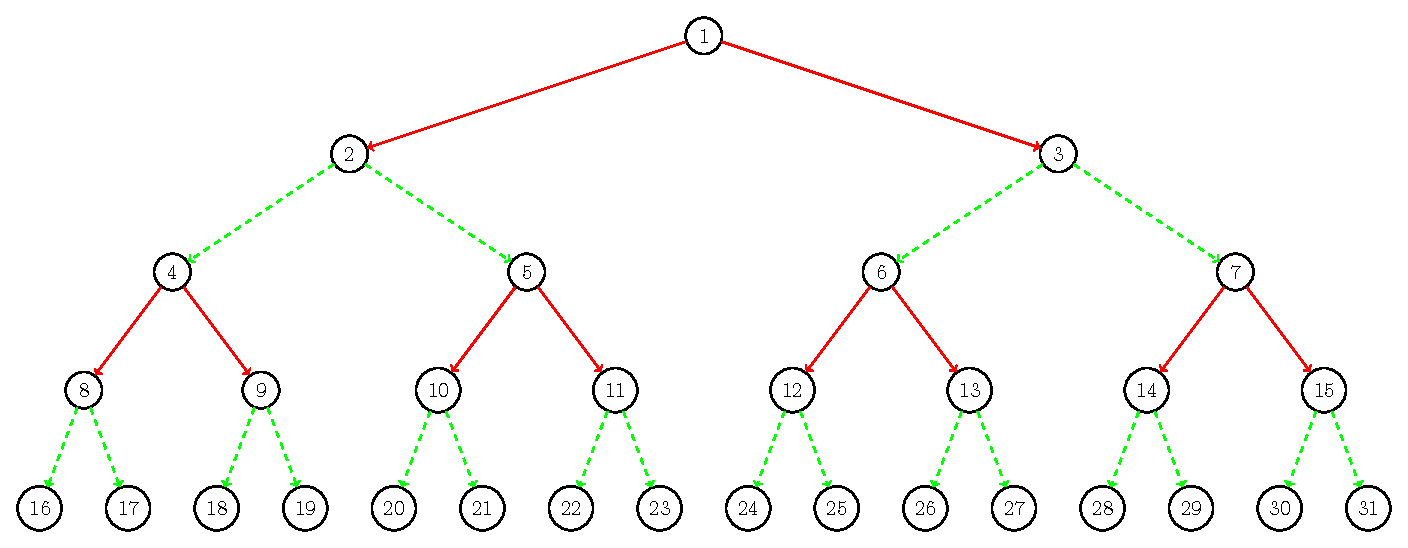
\includegraphics[width=.75\textwidth]{experiment1}
    \caption{Network structure (binary tree) for the first synthetic experiment. The active links of $\mathbf{A}(t)$ alternate between the solid and dashed edges, with extra noise added at each time step, over a period of 10 cycles.}
    \label{fig:exp1}
    \bigskip
\end{figure}

With this experiment, two main objectives are sought. First, to have a better understanding of what role $\alpha$ and $\beta$ parameters play. And second, to confirm that our model captures the cascade effect in the network along a hierarchy of influence that is hidden from a static or aggregate view.

For that purpose, four experiments were run to compute the dynamic broadcast centrality at $t=20$ for each node through \eqref{eqn:u3.3}, varying only the values of both alpha and beta parameters as shown in Table \ref{table:parameters} for each run. Note that the last experimental run does not consider any parameter as it is based on the computation of aggregate measures, in this case, the aggregate out degree represented by row sums of the aggregate adjacency matrix for the whole interval $t=[0,20]$. By analyzing the eigenvalues of all generated $\mathbf{A}_{even}$ and $\mathbf{A}_{odd}$ it is seen that the maximum of the spectral radii of these matrices is 1, and therefore the solution to \eqref{eqn:u3.3} is well defined for $\alpha\in(0,1)$. The SciPy’s \texttt{solve\_ivp} method was used to numerically solve the matrix ODE, which discretizes the time interval in an efficient and transparent way under the hood using the explicit Runge-Kutta method of order 5(4). Relative and absolute tolerances were left to their default values, $atol= 10^{-6}$ and $rtol=10^{-3}$. 

\begin{table}[ht]
            \bigskip
		\centering % used for centering table
		\begin{tabular}{c c c c c} % centered columns (4 columns)
			\hline\hline %inserts double horizontal lines
			\textbf{Parameter} & \textbf{\#1} & \textbf{\#2} & \textbf{\#3} & \textbf{\#4} \\ [0.1ex] % inserts table
			%heading
			\hline\hline 
			$\mathbf{\alpha}$ & 0.7 & 0.7 & 0.1 & -\\ % inserting body of the table
			$\mathbf{\beta}$ & 0.1 & 0.01 & 0.1 & - \\ [0.5ex] % [1ex] adds vertical space
			\hline %inserts single line
		\end{tabular}
		\caption{First synthetic experiment: Choice of the $\alpha,\beta$ parameters for the different experimental runs.} 
       \label{table:parameters} 
\end{table}

Fig. \ref{fig:bt1} displays the dynamic broadcast centrality from \eqref{eqn:u3.4}, at time $t=20$ for each of the 31 nodes for  $\alpha=0.7$ and $\beta=0.1$. We observe that node 1 has a strong advantage in terms of centrality, and that centrality tends to decrease as the index increases. Nodes 2 and 5 are ranked higher than node 3, indicating that the additional noise has affected this part of the network.

Fig. \ref{fig:bt2} depicts the same results with a lower $\beta=0.01$ value, which increases the contribution of older walks. As a reminder, if we consider a walk starting at time zero, then the  downweighting factor becomes $e^{−20 \times 0.01} \approx 0.8$ rather than $e^{−20 \times 0.1} \approx 0.1$. This change of the $\beta$ parameter has a negligible effect on the node rankings which makes sense considering that the network dynamics have an underlying periodic pattern, but it can be observed that it generates larger absolute values.

In Fig. \ref{fig:bt3}, we return to the original $\beta=0.1$ value and set $\alpha$ to 0.1, resulting in less marked differences in the node rankings. Even though node 1 continues to be the most central, the differences are less pronounced as its capability to initiate numerous dynamic walks of length 4 to nodes at the bottom of the hierarchy has less influence or weight.

Fig. \ref{fig:bt4} illustrates the aggregate out degree of each node, that is, the sum of out degrees over time for each node. For nodes 1 to 15 in the binary tree structure, this value is 20 (2 active edges $\times$ 10 cycles), which fluctuates due to the introduced noise. 

Overall, this experiment allows us to clearly visualize the dynamic effect arising from the time-ordering of the node interactions. Due to the hierarchy and timing of the edges, information appears to flow from lower indices to higher. The binary structure of the tree makes node 1 particularly efficient at transmitting information through the network, although this is not immediately apparent in a single snapshot. The last plot highlights that the overall bandwidth in terms of the aggregate out degree of a node can be a misleading network metric for determining node influence.

\begin{figure}[h]
     \centering
     \begin{subfigure}[b]{0.49\textwidth}
         \centering
         \includegraphics[width=\textwidth]{exp1_bt20a}
         \caption{Broadcast for each of the 31 nodes, $\alpha = 0.7 ,~\beta = 0.1$}
         \label{fig:bt1}
     \end{subfigure}
     %\hspace{0.1cm}
     \begin{subfigure}[b]{0.49\textwidth}
         \centering
         \includegraphics[width=\textwidth]{exp1_bt20b}
         \caption{Broadcast for each of the 31 nodes, $\alpha = 0.7 ,~\beta = 0.01$}
         \label{fig:bt2}
     \end{subfigure}
     
     \begin{subfigure}[b]{0.49\textwidth}
         \centering
         \includegraphics[width=\textwidth]{exp1_bt20c}
         \caption{Broadcast for each of the 31 nodes, $\alpha = 0.1 ,~\beta = 0.1$}
         \label{fig:bt3}
     \end{subfigure}
     %\hspace{0.1cm}
     \begin{subfigure}[b]{0.49\textwidth}
         \centering
         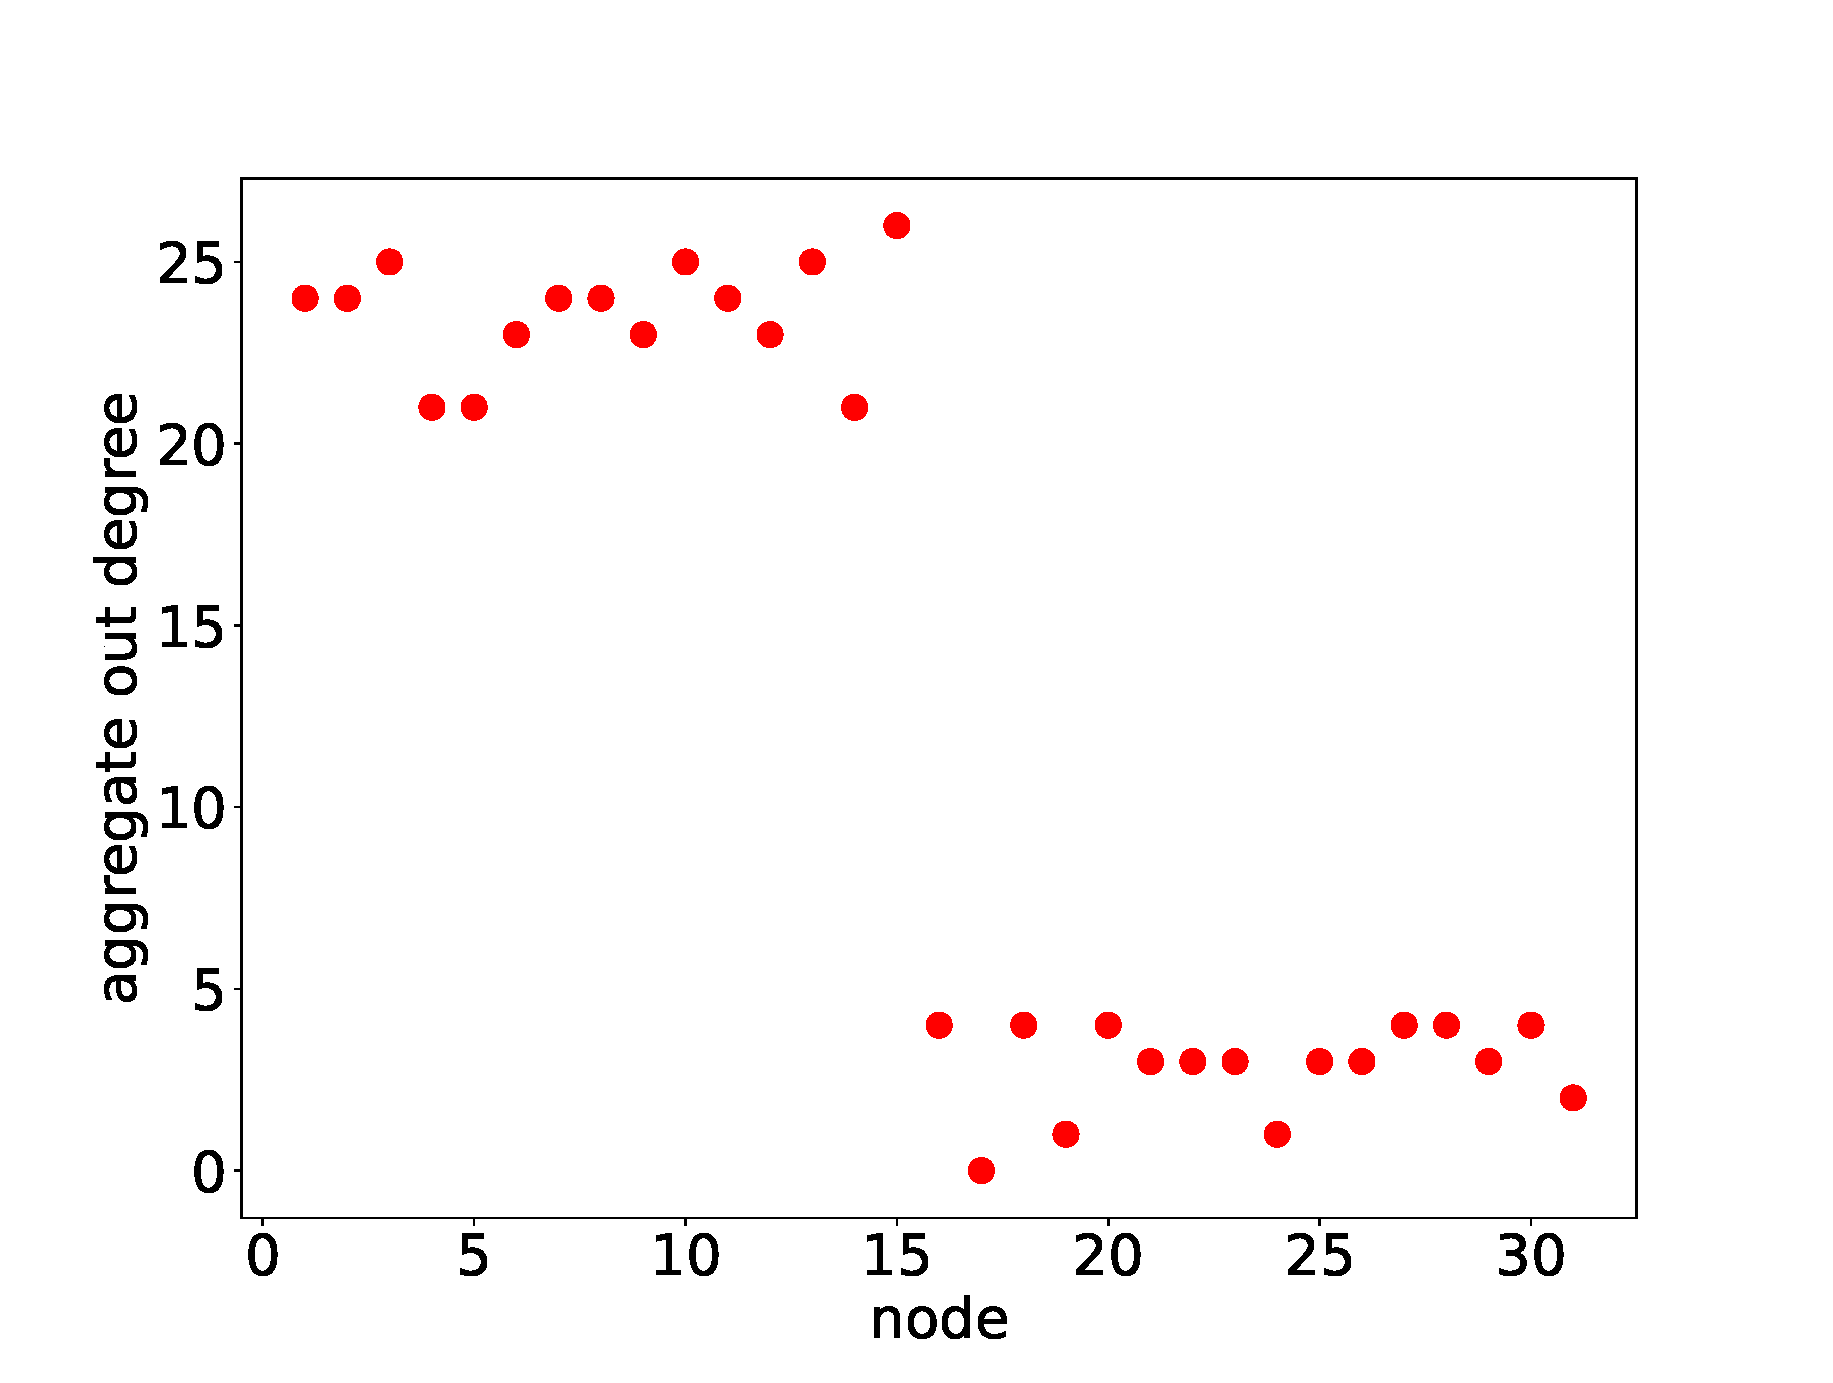
\includegraphics[width=\textwidth]{exp1_agg_out_degree}
         \caption{Aggregate out degree for each node}
         \label{fig:bt4}
     \end{subfigure}
        \caption{First synthetic experiment: results from the dynamic network in Fig. \ref{fig:exp1}.}
        \label{fig:fourbt}
\end{figure}

\newpage
\section{Second synthetic experiment}
\label{sec:synexp2}
We now consider the second synthetic experiment from \cite{grindrod2014dynamical}. The experiment simulates multiple rounds of voice calls that occur along an undirected binary tree structure. Each node in the tree has at most one active edge at any given time, meaning that there are no "conference" calls. Fig. \ref{fig:exp2} shows the network of $N=17$ nodes with labels assigned to the edges indicating when they are active. The adjacency matrix, $\mathbf{A}(t)$, for this experiment is defined based on the ordered and non-overlapping time intervals such that $t_i\coloneqq[(i − 1)\tau , (i − 1 + 0.9)\tau )$, for $i=0, 1, \dots , 7$, and $\tau =0.1$.

\begin{figure}[h]\centering
    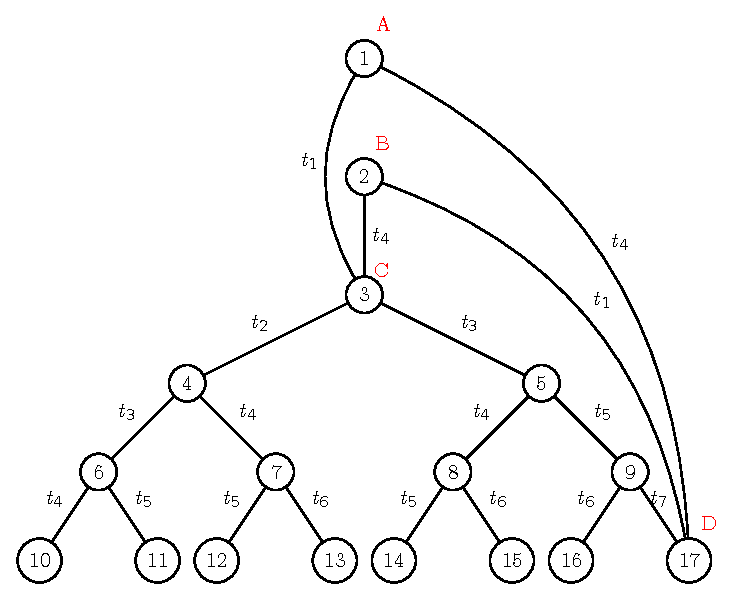
\includegraphics[width=.65\textwidth]{experiment2}
    \caption{Network structure for the second synthetic experiment. Links of $\mathbf{A}(t)$ are active over non-overlapping time intervals such that $t_i\coloneqq[(i − 1)\tau , (i − 1 + 0.9)\tau )$, for $i=0, 1, \dots , 7$, and $\tau =0.1$, repeated periodically over five cycles.}
    \label{fig:exp2}
    \bigskip
\end{figure}

The dynamic network is constructed in a way that node A (node 1) is designed to be a more effective influencer compared to node B (node 2). This can be attributed to several factors such as a higher social/business status or access to more current and relevant information. Connections are built in such a way that node A talks to node C (node 3) in $t_1$, initiating a cascade of phone calls in the network. On the other hand, node B communicates with node D (node 17) at $t_1$ and waits until $t_4$ to contact node C, which does not trigger any new cascades. The experiment is repeated over five cycles, during which nodes A and B send out a total of 10 messages. 

What we expect from this experiment, and makes it different from the previous one, is to verify that our continuous-time framework is capable of revealing the differences in terms of dynamic broadcast centrality between the node A that enjoys a cascade effect of information in the network and node B that does not. Even if these nodes have an apparent identical behaviour from an overall perspective, both contacting nodes C and D for the same length of time.

As pointed out in the remark on the role of the $\alpha$ and $\beta$ parameters, in the scenario of undirected one-to-one communication, such as voice calls with no tele-conferences, all the symmetric adjacency matrices turn out to have unitary spectral radius for each time interval. A complete definition of these matrices can be seen in Appendix \ref{sec:fse} - Second synthetic experiment, l.22. Values of $\alpha=0.7$ and $\alpha=0.9$ were chosen to compare centrality results keeping fixed the value of $\beta=0.1$ which does not play an important role in this experiment due to the underlying periodic pattern in the network dynamics (similar results were obtained for different values of $\beta$). 

Implementing \eqref{eqn:u3.3}--\eqref{eqn:u3.4} in Python, $\mathbf{b}(t)$ was computed for the interval $t=[0,3.5]$ for nodes A and B, using the \texttt{solve\_ivp} function with default parameters: method="RK45", $atol=10^{-6}$ and $rtol=10^{-3}$.

The results in Fig. \ref{fig:twobt} (for $\alpha = 0.7, \beta = 0.1$ and $\alpha = 0.9 , \beta = 0.1$ respectively) show that the dynamic broadcast centrality measure is able to capture the cascade effect enjoyed by node A (solid line) with respect to node B (dashed line). This difference in broadcast centrality is much more pronounced for values of $\alpha$ close to one (Fig. \ref{fig:bt6}), where longer walks are more strongly penalized. 

\begin{figure}
     \centering
     \begin{subfigure}[b]{0.49\textwidth}
         \centering
         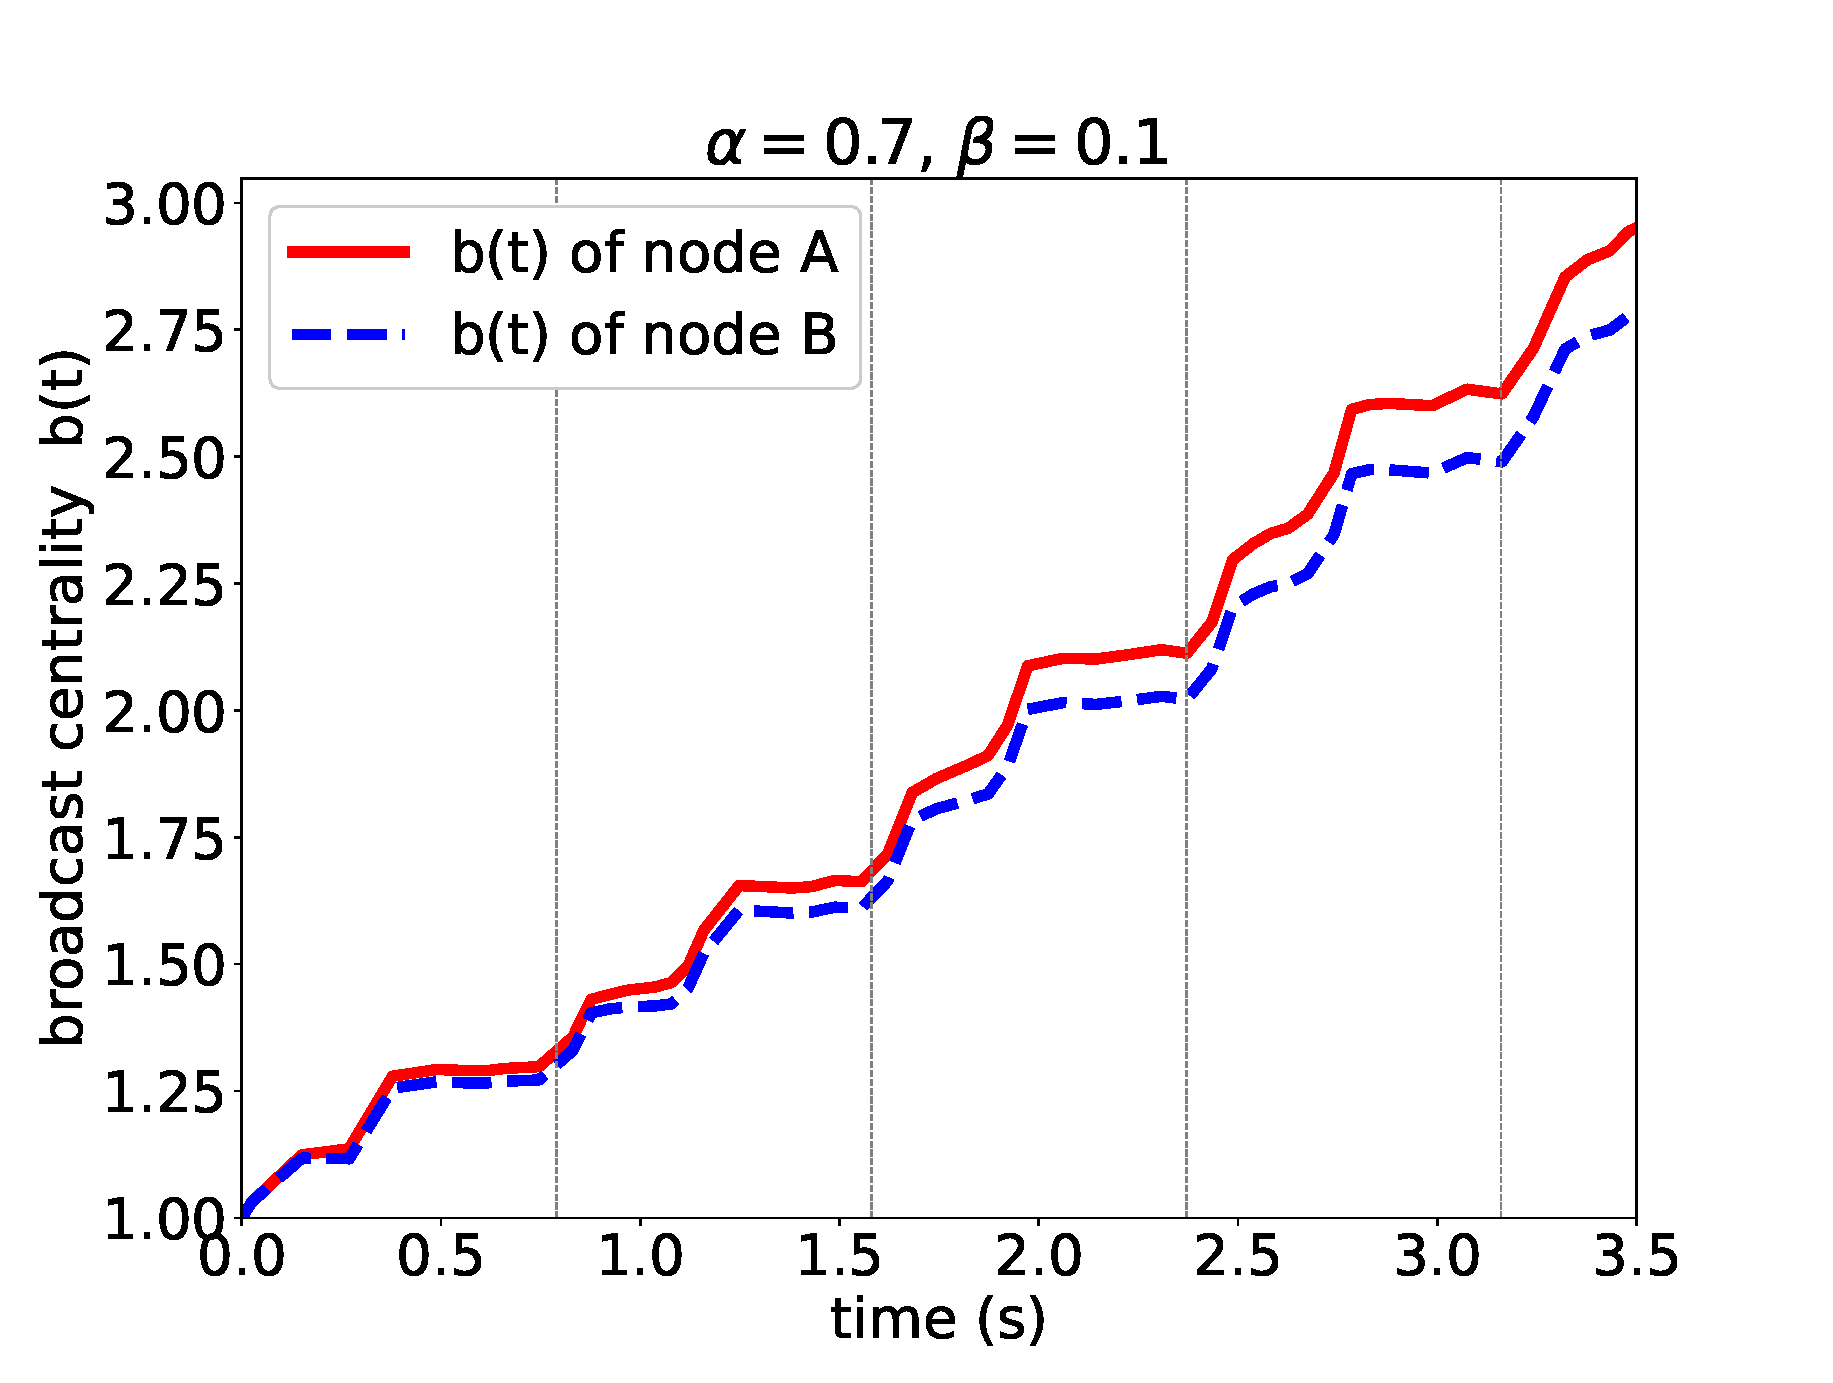
\includegraphics[width=\textwidth]{exp2b_btA_vs_btB}
         \caption{$\mathbf{b}(t)$ for $\alpha = 0.7 ,~\beta = 0.1$}
         \label{fig:bt5}
     \end{subfigure}
     \hfill
     \begin{subfigure}[b]{0.49\textwidth}
         \centering
         \includegraphics[width=\textwidth]{exp2a_btA_vs_btB}
         \caption{$\mathbf{b}(t)$ for $\alpha = 0.9 ,~\beta = 0.1$}
         \label{fig:bt6}
     \end{subfigure}
     \caption{Second synthetic experiment: dynamic broadcast centrality over time for node A (solid) and node B (dashed) in the network of Fig. \ref{fig:exp2}.}
     \label{fig:twobt}
\end{figure}

The iterative way in which the dynamic communicability matrix \eqref{eqn:dyncommatiter} is defined as a product of non-negative matrices based on the computation of the previous steps, ensures that nodes do not become less communicative over time. This characteristic is reflected in the increasing curves for both plots. This can also be interpreted from the fact that as time goes on, more nodes in the network will have received the message. Then, as more nodes receive the message, the number of nodes that can be reached in a single step will increase, and so will the broadcast centrality of the original node. Moreover, if we divide the plots into the five cycles that network communication is repeated by vertical lines, the particular staircase shape of the curves is explained by the fact that nodes A and B are active during $t_1$ and $t_4$ which causes a notable increase in broadcast centrality after these points.

As a curiosity, other nodes in this network, such as nodes 3, 4 and 5, offer greater centrality than nodes 1 (node A) and node 2 (node B). In fact, node 3 is the one with the highest centrality in the entire network. However, the main objective of this experiment was not to highlight this feature but to verify that our continuous-time ODE framework was capable of establishing a remarkable difference in the dynamic behavior between nodes A and B.

\newpage

\section{Voice call experiment}
\label{sec:voicecall}
The next experiment applies the new modelling framework \eqref{eqn:u3.3} to a set of voice call interactions, in order to analyze the dynamic behavior of a fictitious, controversial socio-political movement. The data used for the experiment, supplied as part of the IEEE VAST 2008 Challenge \cite{grinstein2008vast}, consists of a complete set of 9834 time-stamped calls across 400 cell phone users over a 10 day period, with information on IDs for the send and receive nodes, start time in hours/minutes, and duration in seconds.

The aim of the experiment is to show the usefulness of the new matrix ODE in dealing with this type of dynamic network, comparing dynamical measures against aggregated. To that end, the bandwidth of a node is defined as the aggregate number of seconds for which the node ID is active as a sender or receiver. This will allow us to compare the effective activation time of a certain node with its relevance in terms of dynamic broadcast centrality.

The designers of the above mentioned competition provided additional information indicating that node 200 was the leader of an important community who controlled a closely connected subnetwork or inner circle consisting of nodes 1, 2, 3, and 5. However, starting from day 7, these individuals seem to have switched their phone IDs: node 200 became 300, and the others became 306, 309, 360, and 392.

For this experiment, $\mathbf{A}(t)$ was assumed to be symmetric, meaning that $\mathbf{A}_{ij}(t) = \mathbf{A}_{ji}(t) = 1$ if nodes $i$ and $j$ were communicating at time $t$, which was measured in seconds. Parameters $\beta$ was chosen to be approximately $\beta = 1/(60\times 60 \times 24) \approx 1.2 \times 10^{-5}$, which corresponded to a time downweighting of $e^{-1}$ per day, and set the edge attenuation parameter $\alpha$ to a similar value of $10^{-4}$. The SciPy's \texttt{solve\_ivp} method was again used to numerically solve the ODE (\ref{eqn:u3.3}) (see Appendix \ref{chap:appa} - Voice call experiment, l.257). Additionally, absolute and relative error tolerances were both set to $10^{-4}$. To improve efficiency, the matrix logarithm was approximated in this occasion with its expansion to the fifth power:

$$\log(\mathbf{I} - \alpha \mathbf{A}(t)) \approx \alpha \mathbf{A}(t) - \alpha^2 \mathbf{A}(t)^2/2 + \alpha^3 \mathbf{A}(t)^3/3 - \alpha^4 \mathbf{A}(t)^4/4 + \alpha^5 \mathbf{A}(t)^5/5$$ 

Visually speaking, the effects of increasing the number of terms in the expansion to 6 and 7 remained identical.

\begin{figure}[h]\centering
    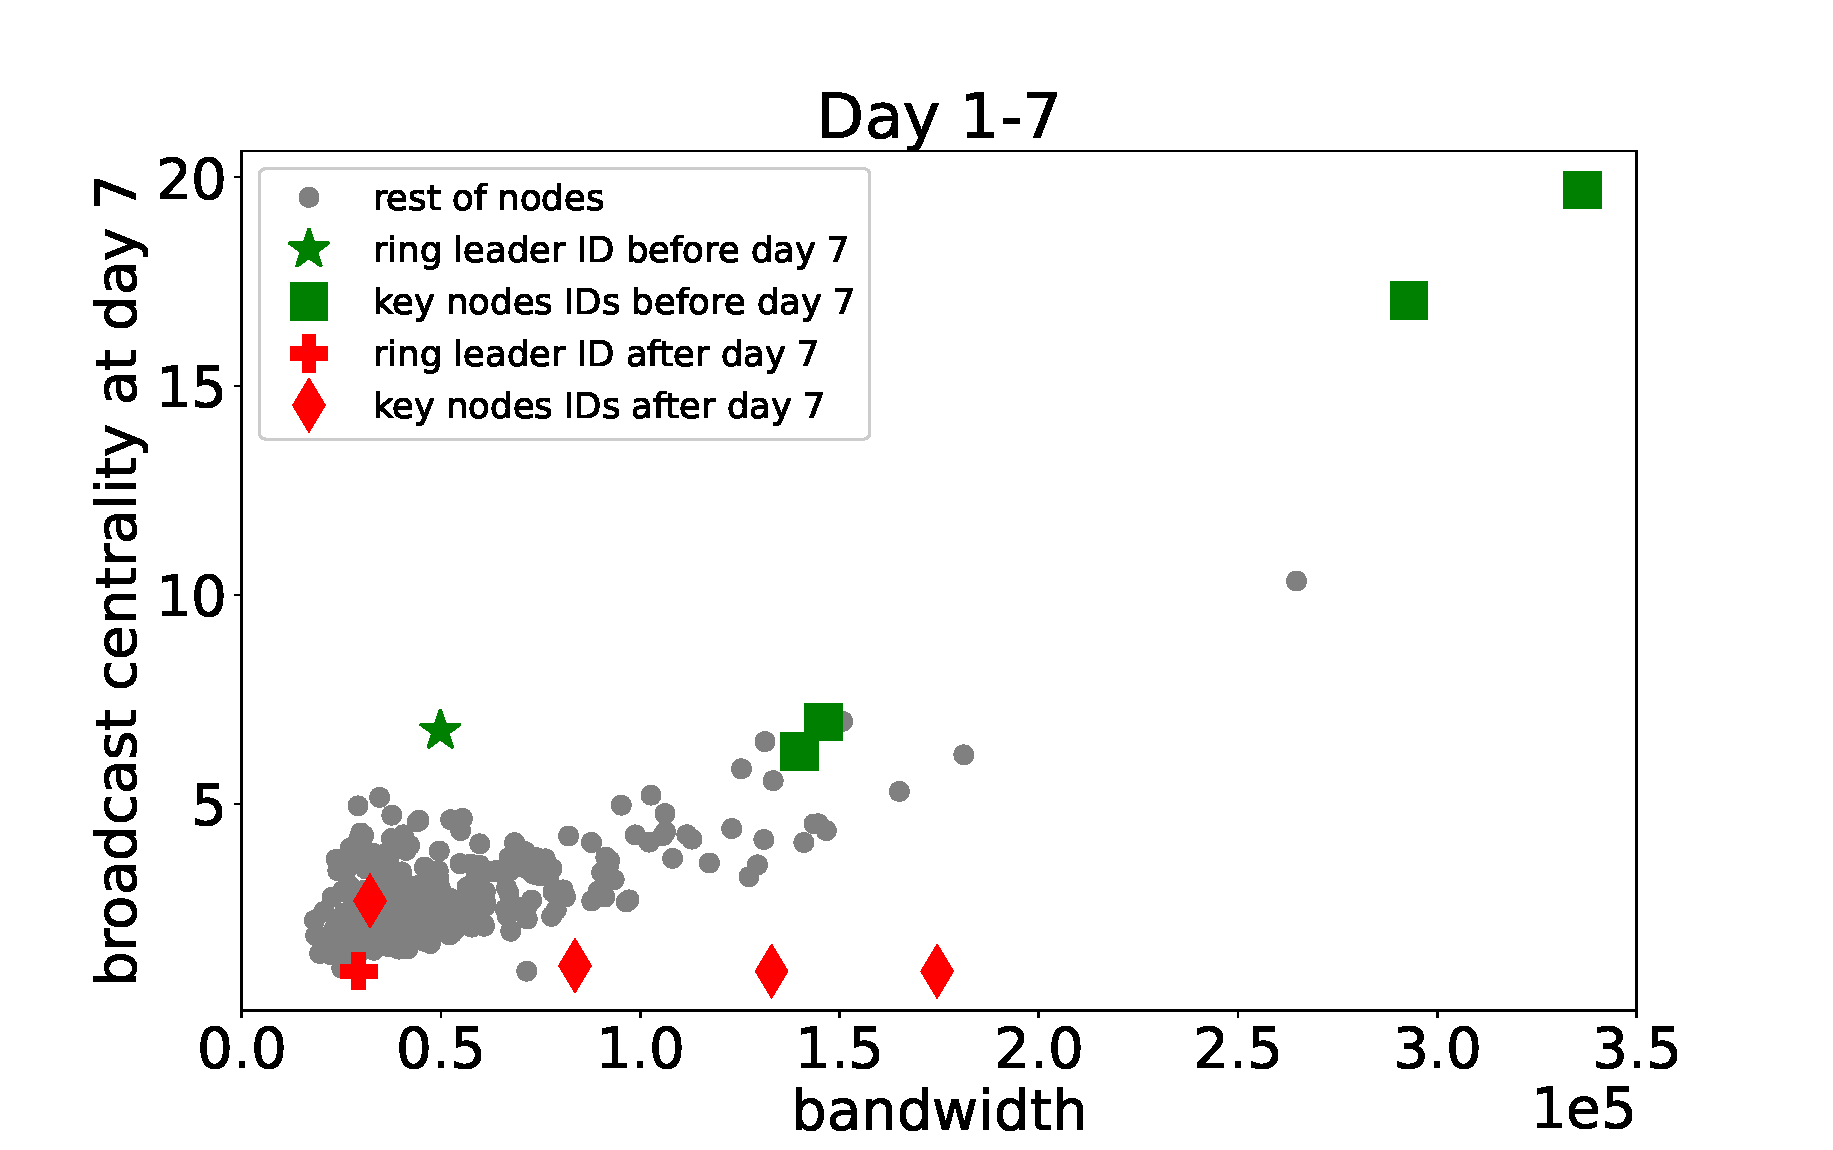
\includegraphics[width=.79\textwidth]{voicecall_exp_1_7}
    \caption{Voice call experiment: broadcast centrality for each node at the end of day 6 vs. bandwidth (secs.).}
    \label{fig:ve1a}
    \bigskip
\end{figure}

This experiment yields two key findings:
\begin{enumerate}[label=(\roman*)]
  \item The dynamic broadcast/receive measures \eqref{eqn:u3.4} are able to identify key nodes as highly influential, even if they are not actively using much bandwidth, without any prior knowledge of an inner circle's existence.
  \item The transformation that occurs in the network on day 7 is revealed by the running centrality measures once we know the IDs of the inner circle.
\end{enumerate}

Fig. \ref{fig:ve1a} was used to demonstrate point (i) by plotting bandwidth against dynamic broadcast, $\mathbf{b}(t)$, using data up until the end of day 6. The scatter plot also includes symbols to mark certain nodes, such as a star for the ring leader, 200, and squares for the related inner-circle nodes, 1, 2, 3, and 5. The follow-on ID for the ringleader, 300, is marked with a plus symbol, and those for other members, 306, 309, 360, and 392, are marked with diamonds.

The results showed that the key nodes for days 1-6 were much more dominant in terms of dynamic broadcast than overall bandwidth. Specifically, the ringleader node had a low bandwidth but ranked sixth out of 400 in terms of broadcast communicability.

\begin{figure}[h]\centering
    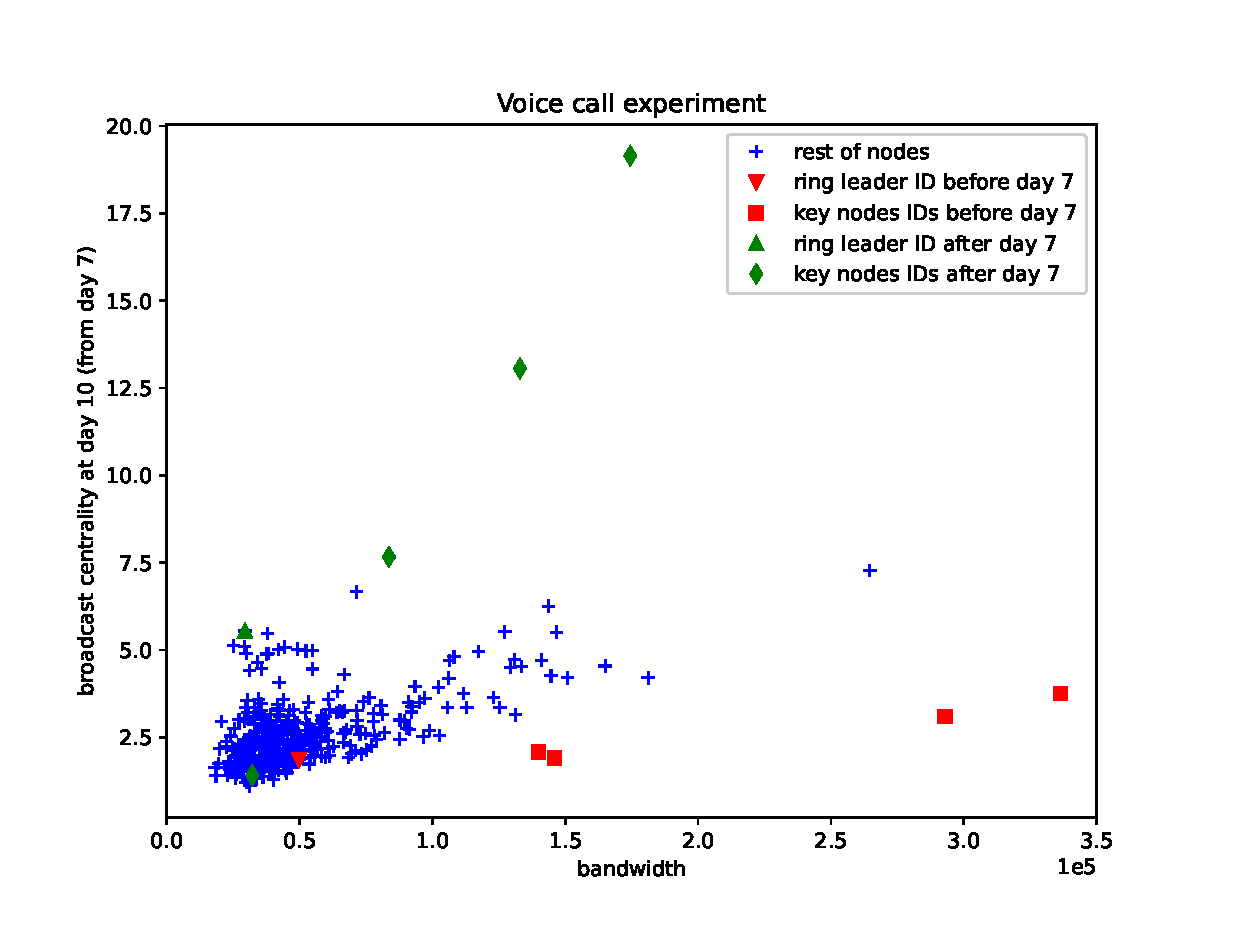
\includegraphics[width=.79\textwidth]{voicecall_exp_7_10}
    \caption{Voice call experiment: broadcast centrality for each node at the end of day 10 vs. bandwidth (secs.).}
    \label{fig:ve1b}
    \bigskip
\end{figure}

The data from days 7 to 10 is displayed in Fig. \ref{fig:ve1b}. The plot shows how the new ID of the ringleader, that is indicated by a plus symbol, has a low overall bandwidth, but ranks seventh highest for broadcast centrality. Although the former IDs from the inner circle, marked with diamonds, still possess high bandwidth, their low dynamic broadcast scores suggest that they are no longer central players. This experiment confirms that the dynamic broadcast score is a more effective indicator of centrality than overall bandwidth in uncovering the inner circle.

Dynamic receive centrality, $\mathbf{r}(t)$, was also computed using its own vector-valued ODE \eqref{eqn:u4.1} for data from days 1 to 7 obtaining similar results and a computation time reduction per function call of approximately $30\%$ (see Appendix \ref{chap:appa} - $\mathbf{b}(t)$ vs. $\mathbf{r}(t)$ cost comparison). The execution times in the $\mathbf{b}(t)$ vs. $\mathbf{r}(t)$ comparison have been measured over 100 repetitions for the computation of the respective matrix/vector ODE system. We determined the frequency (time per call ratio) at which the matrix function \eqref{eqn:u3.3} or vector function \eqref{eqn:u4.1} was evaluated by the \texttt{solve\_ivp} Python method with default parameters. Results are shown in Table \ref{table:btrt}.

\begin{table}[ht]
            \bigskip
		\centering % used for centering table
		\begin{tabular}{c c c c} % centered columns (4 columns)
			\hline\hline %inserts double horizontal lines
			\textbf{Method ($\times 100$ rep.)} & \textbf{time (s)} & \textbf{function calls} & \textbf{ratio (ms/call)} \\ [0.1ex] % inserts table
			%heading
			\hline\hline 
			$\mathbf{b}(t)$ & 984.47 & 32600 & 30.20 \\ % inserting body of the table
			$\mathbf{r}(t)$ & 2627.48 & 122600 & 21.43 \\ [0.5ex] % [1ex] adds vertical space
			\hline %inserts single line
		\end{tabular}
		\caption{$\mathbf{b}(t)$ vs. $\mathbf{r}(t)$ cost comparison.} 
       \label{table:btrt} 
\end{table}

We define the \textit{communicability between key nodes ($\mathcal{C}$)} at each discretized time point, as the average amount of messages, broadcast ($U_{ij}$) and received ($U_{ji}$), between each pair of key nodes, scaled by the average amount of communication between all pairs of nodes in the network, i.e.,

\begin{equation*}
    \mathcal{C}(t) = \frac{\overline{K}(t)}{\overline{T}(t)},
\end{equation*}

where

\begin{align*}
    \overline{K}(t) &=\frac{\sum_{i\ne j}U_{ij}(t) + U_{ji}(t)}{20} \text{~~~~~for~~} i=1,2,3,5,200 ,\\
    \overline{T}(t) &=\frac{\sum_{i,j=1}^N U_{ij}(t) - \sum_{i=1}^N U_{ii}(t)}{N^2-N}.
\end{align*}

The communicability between the original IDs of the five most important players (ID nodes: 200, 1, 2, 3, and 5) during the ten days period is presented in Figure \ref{fig:ve2} to support point (ii). By analyzing this measure, we can observe how the structure of the network changes over time, especially when the players start using different IDs after day 7.

\begin{figure}[h]\centering
    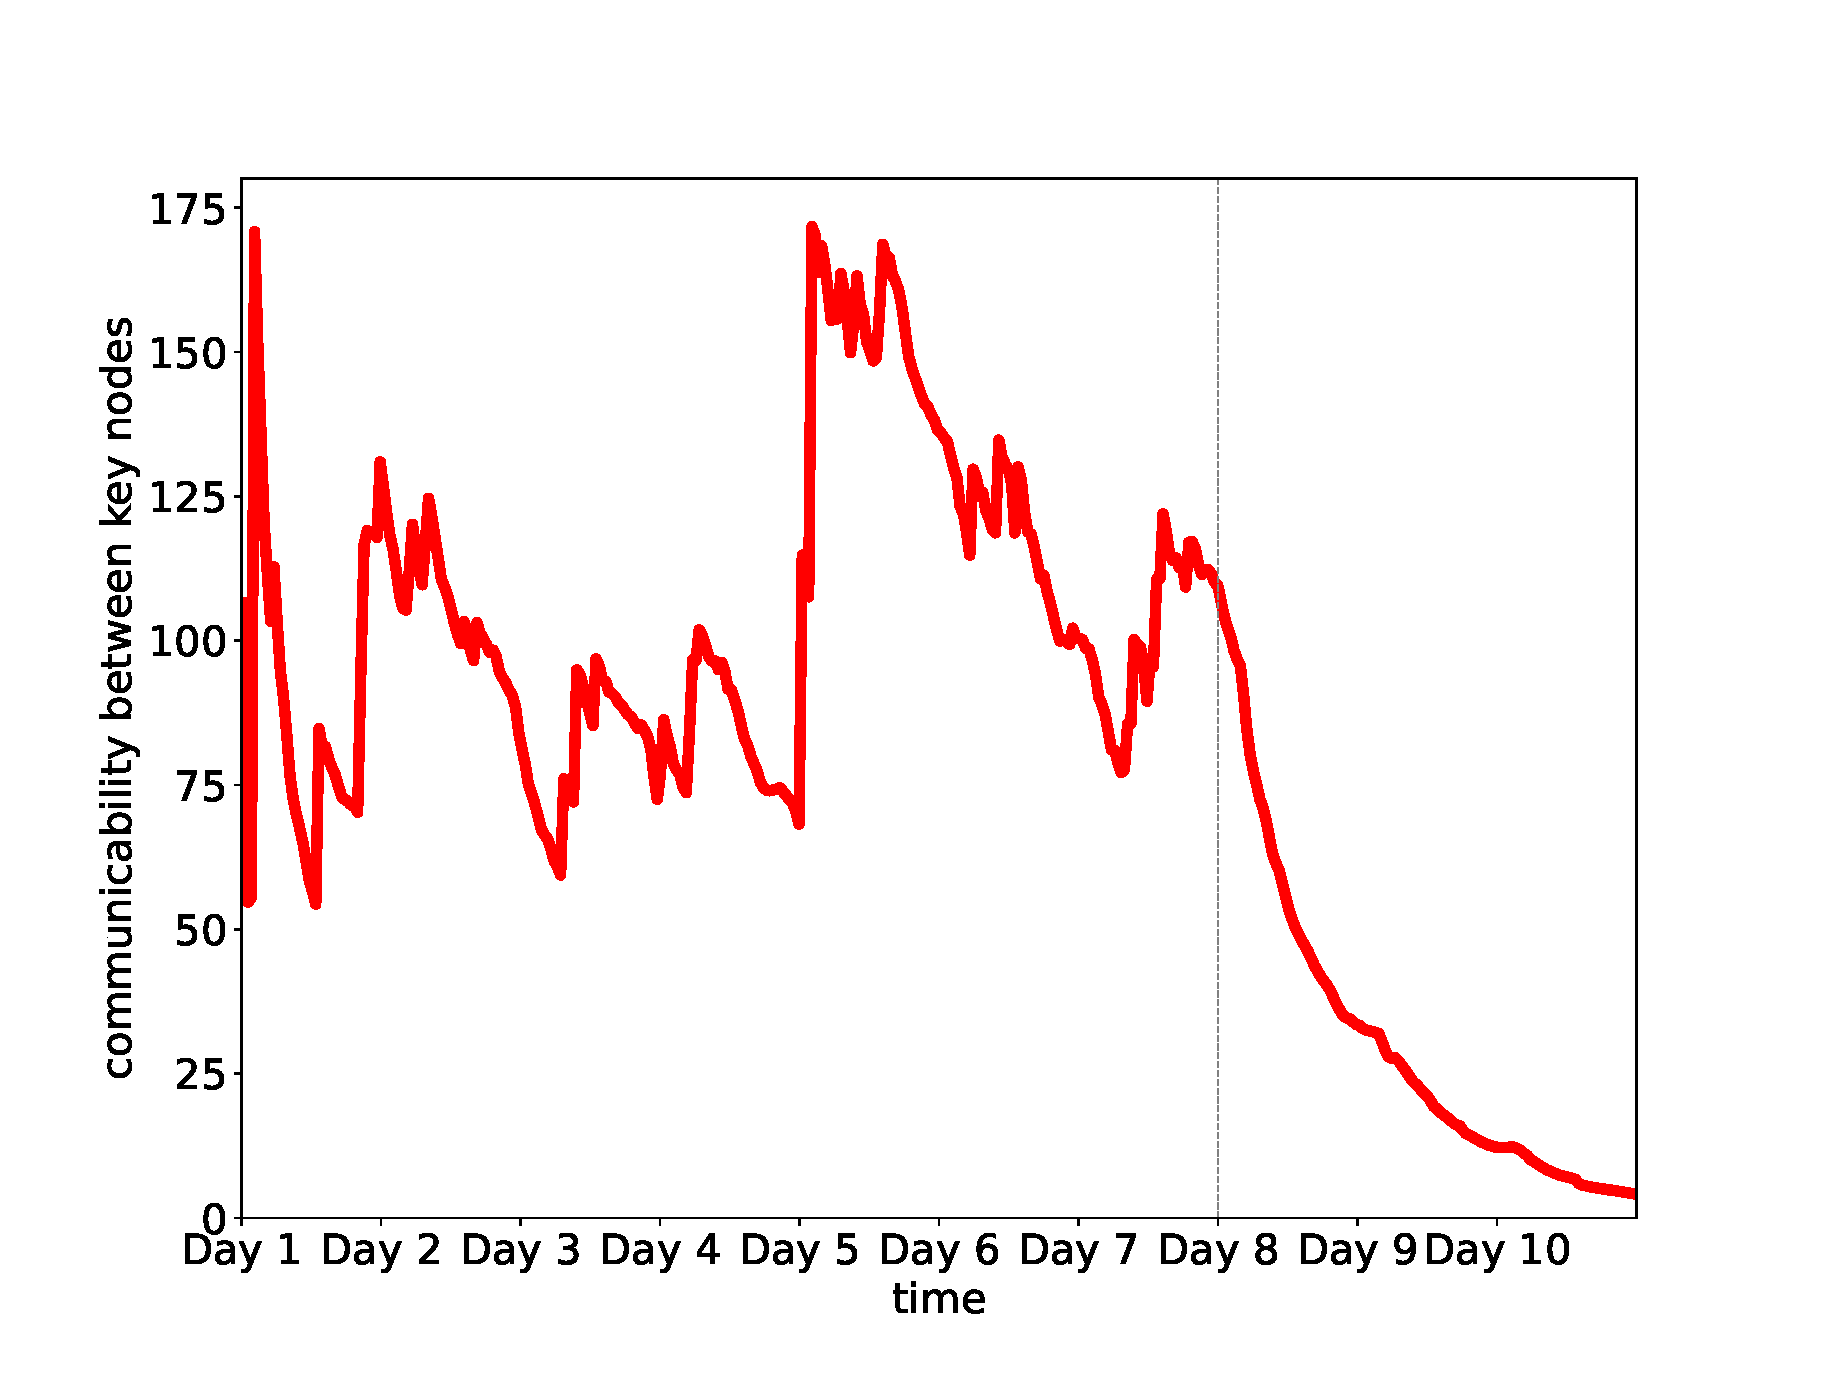
\includegraphics[width=.85\textwidth]{voicecall_exp_dyncomm}
    \caption{Voice call data: dynamic communicability between the five key nodes as a function of time.}
    \label{fig:ve2}
    \bigskip
\end{figure}  
	
	% ----------------------------------------------------------------------------------
% ----------------------------------------------------------------------------------

\chapter{Conclusions}
\label{chap:concl}

Text.




 % CONCLUSIONS

    % ----------------------------------------------------------------------------------
% ----------------------------------------------------------------------------------

\chapter{Further studies}
\label{chap:further}

\begin{highlightedParagraphC}
 
Further generalization of the framework on dynamical systems at lower dimensions.

\end{highlightedParagraphC}

A natural continuation of this study could be applied to different types of dynamical systems where only a few nodes compared to the total number of nodes are really significant in the behavior and evolution of such systems. For instance, consider an evolving network $\mathbf{A}(t)$ with $N \times N$ dimensions, where $N$ is very large. If a smaller subset of $M\ll N$ nodes is identified as significant, it might be worthwhile to explore an ordinary differential equation involving $V(t)\in \mathbb{R}^{M\times M}$ with $M\times M$ dimensions. The equation could be in the form of 

$$V(t)=P(V(t)) + Q(V(t))F(A(t)),$$ where $P$ and $Q$ are polynomial or matrix-valued functions, and $F: [0, 1]^{N×N} \to \mathbb{R}^{M\times M}$ is an appropriate matrix-valued mapping. This kind of system would allow us to reduce the interactions among all $N$ nodes to the subset of interest, and then measure the resulting changes in behavior in this lower dimension.

\begin{highlightedParagraphC}
 
Potential use of the framework in applied scientific fields.

\end{highlightedParagraphC}

Further studies could explore the potential of centrality measures such as the generalized Katz measure derived from this study and dynamic network broadcast/receive analysis in applied fields like fluid dynamics, atmosferic science or engineering: 

\begin{itemize}
  \item These measures could be used to study the complex spatiotemporal dynamics of turbulent flows, and identify key locations or structures that could be targeted for control or optimization. 
  \item They can also be a useful tool in the study of fluid combustion, by identifying the critical points in the combustion system where the combustion reaction is most likely to be affected by various factors such as temperature, pressure, and turbulence. This information can be used later to optimize the combustion process and improve its efficiency.
\end{itemize}
	
Many other scientific areas are suitable to the application of this novel framework such as social networks, traffic flow, transportation or power grids, neural networks... since a huge number of real problems can be modeled through the use of evolving networks.

Overall, the application of centrality measures has the potential to provide valuable insights into the behavior of complex systems in multiple and diverse fields, enabling the development of more effective control and optimization strategies. % FURTHER STUDIES
	
	%% ----------------------------------------------------------------------------------
% ----------------------------------------------------------------------------------

\chapter{Conclusions}
\label{chap:concl}

Text.




  
	
	% -------------------------------------------------------
	% -------------------------------------------------------
	% -------------------------------------------------------
	% BIBLIOGRAPHY
	
	\bibitemsep = 3ex
	\bibhang = 2em
	
	%\nocite{*} %includes ALL refs in the bibliographic database whether or not were cited in the text
	
	\printbibliography[heading=bibintoc,title=\bibname]
	
	% -------------------------------------------------------
	% Appendices
	
	\clearpage
	\pagenumbering{arabic}% resets `page` counter to 1
	\renewcommand*{\thepage}{A\arabic{page}}
	
	\begin{appendices}
		\chapter{$\vert$ Python code}
\label{chap:appa}

\section*{First synthetic experiment}
\label{sec:fse}

\begin{lstlisting}[language=Python, caption=First synthetic experiment]
#!/usr/bin/env python3
# -*- coding: utf-8 -*-

#############################################################
################### SYNTHETIC EXPERIMENT 1 ##################
#############################################################

########################## MODULES ##########################

import numpy as np
from scipy.integrate import solve_ivp
from scipy.linalg import logm
import matplotlib.pyplot as plt

######################### VARIABLES #########################
# number of nodes
N = 31 
# alpha and beta parameters
a = 0.7
b = 0.1
# depth of binary tree (2 even and 2 odd)
levels = 2
# identity matrix
I = np.eye(N) 

######################### FUNCTIONS #########################

def unirandom(matrix):
    '''
    Introduces a 1 in a uniform randomized number of entries, specified by the 
    parameter 'num_entries' in a given matrix.

            Parameters:
                    matrix (arr): matrix of size MxN

            Returns:
                    -
    '''
    # number of entries to randomize, uniform dist. with avg.= 5
    num_entries = int(np.random.uniform(low=0, high=10))
    
    if matrix.size < num_entries:
        raise ValueError("Invalid number of entries to randomize")
        
    # randomly select num_entries unique positions in the matrix
    positions = np.random.choice(matrix.size, size=num_entries, replace=False)
    # set the selected positions to 1
    matrix.flat[positions] = 1.

def A_even():
    '''
    Returns the constant value that takes A(t) at even time intervals with 
    some noise added by 'unirandom' function.

            Parameters:
                    -

            Returns:
                    ematrix (arr): NxN matrix for even time intervals
    '''
    ematrix = np.zeros((N, N))
    for i in (2**k for k in range(0, levels*2 , 2)):
        for j in range(1, i+1):
            ematrix[i-1][i*2-1] = 1
            ematrix[i-1][i*2] = 1
            i = i + 1
    unirandom(ematrix)
    return ematrix

def A_odd():
    '''
    Returns the constant value that takes A(t) at odd time intervals with 
    some noise added by 'unirandom' function.

            Parameters:
                    -

            Returns:
                    omatrix (arr): NxN matrix for odd time intervals
    '''
    omatrix = np.zeros((N, N))
    for i in (2**k for k in range(1, levels*2 , 2)):
        for j in range(1, i+1):
            omatrix[i-1][i*2-1] = 1
            omatrix[i-1][i*2] = 1
            i = i + 1
    unirandom(omatrix)
    return omatrix
   
def aggregate_out_degree(matrix):
    '''
    Returns the row sums that represent the aggregate out degree for each
    node (row) given an adjacency matrix.

            Parameters:
                    matrix (arr): adjacency matrix of size NxN

            Returns:
                    row_sums (list): list of agg. out degree for each node
    '''
    row_sums = [sum(row) for row in matrix]
    
    return row_sums


######################### A(t) #########################

# time interval t=[0, 20], with A(t) constant over each subinterval [i, i + 1)
# where A(t) = A_even and A(t) = A_odd when 'i' is even and odd respectively

A0 = A_even()
A1 = A_odd()
A2 = A_even()
A3 = A_odd()
A4 = A_even()
A5 = A_odd()
A6 = A_even()
A7 = A_odd()
A8 = A_even()
A9 = A_odd()
A10 = A_even()
A11 = A_odd()
A12 = A_even()
A13 = A_odd()
A14 = A_even()
A15 = A_odd()
A16 = A_even()
A17 = A_odd()
A18 = A_even()
A19 = A_odd()
A20 = np.zeros((N, N))

w0, v0 = eig(A0)
w1, v1 = eig(A1)
w2, v2 = eig(A2)
w3, v3 = eig(A3)
w4, v4 = eig(A4)
w5, v5 = eig(A5)
w6, v6 = eig(A6)
w7, v7 = eig(A7)
w8, v8 = eig(A8)
w9, v9 = eig(A9)
w10, v10 = eig(A10)
w11, v11 = eig(A11)
w12, v12 = eig(A12)
w13, v13 = eig(A13)
w14, v14 = eig(A14)
w15, v15 = eig(A15)
w16, v16 = eig(A16)
w17, v17 = eig(A17)
w18, v18 = eig(A18)
w19, v19 = eig(A19)

print("w0 =", w0)
print("w1 =", w1)
print("w2 =", w2)
print("w3 =", w3)
print("w4 =", w4)
print("w5 =", w5)
print("w6 =", w6)
print("w7 =", w7)
print("w8 =", w8)
print("w9 =", w9)
print("w10 =", w10)
print("w11 =", w11)
print("w12 =", w12)
print("w13 =", w13)
print("w14 =", w14)
print("w15 =", w15)
print("w16 =", w16)
print("w17 =", w17)
print("w18 =", w18)
print("w19 =", w19)

# aggregate matrix to compute the agg. out degree
agg_matrix = A0 + A1 + A2 + A3 + A4 + A5 + A6 + A7 + A8 + A9 + A10 +\
             A11 + A12 + A13 + A14 +A15 + A16 + A17 + A18 + A19
      

# Adjacency matrix for t=[0,20]
def Adj(t):
    if 0.0 <= t < 1.0:
        return A0
    if 1.0 <= t < 2.0:
        return A1
    if 2.0 <= t < 3.0:
        return A2
    if 3.0 <= t < 4.0:
        return A3
    if 4.0 <= t < 5.0:
        return A4
    if 5.0 <= t < 6.0:
        return A5
    if 6.0 <= t < 7.0:
        return A6
    if 7.0 <= t < 8.0:
        return A7
    if 8.0 <= t < 9.0:
        return A8
    if 9.0 <= t < 10.0:
        return A9
    if 10.0 <= t < 11.0:
        return A10
    if 11.0 <= t < 12.0:
        return A11
    if 12.0 <= t < 13.0:
        return A12
    if 13.0 <= t < 14.0:
        return A13
    if 14.0 <= t < 15.0:
        return A14
    if 15.0 <= t < 16.0:
        return A15
    if 16.0 <= t < 17.0:
        return A16
    if 17.0 <= t < 18.0:
        return A17
    if 18.0 <= t < 19.0:
        return A18
    if 19.0 <= t <= 20.0:
        return A19
    return A20
    
######################### ODE #########################

# Matrix ODE function in vector form
def f(t, U):
    
    # Reshape U from vector to matrix
    U = U.reshape((N, N))
    
    # Compute the matrix ODE
    dUdt = -b * (U - I) - U @ logm(I - a * Adj(t))
    
    # Reshape dUdt from matrix to vector
    dUdt = dUdt.flatten()
    return dUdt


# Initial condition 
U0 = np.eye(N)
U0 = U0.flatten()
#time span
t_span = (0, 20)

# Solve the matrix ODE numerically using Runge-Kutta 45 method
sol = solve_ivp(f, t_span, U0, method='RK45')

# Print the solution at discrete time points
print("\nsol_t :\n", sol.t)
print("\nsol_y :\n", sol.y)

# Communicability matrix U at t = 20 (entries >= 0)
U_t_20 = np.abs(sol.y[:,-1].reshape(N,N))

# broadcast centrality at t = 20
b_t_20 = U_t_20 @ np.ones(N)

# aggregate out degree 
out_degree_list = aggregate_out_degree(agg_matrix)

print("\nb(t=20) :\n", b_t_20)
print("\nAgg. out degree =", out_degree_list)

######################### PLOTS #########################

fig, ax = plt.subplots()
ax.plot(list(range(1,N+1)), b_t_20, '*')
ax.set_title(r"First synthetic experiment: $\alpha=0.7$ $\beta=0.1$")
ax.set_xlabel("node")
ax.set_ylabel("dynamic broadcast  b(t=20)")

fig.savefig('exp1_bt20.eps', format='eps')

fig2, ax2 = plt.subplots()
ax2.plot(list(range(1,N+1)), out_degree_list, '*', color='r')
ax2.set_title("First synthetic experiment")
ax2.set_xlabel("node")
ax2.set_ylabel("aggregate out degree")

fig2.savefig('exp1_agg_out_degree.eps', format='eps')
\end{lstlisting}

\section*{Second synthetic experiment}
\label{sec:sse}

\begin{lstlisting}[language=Python, caption=Second synthetic experiment]
#!/usr/bin/env python3
# -*- coding: utf-8 -*-

#############################################################
################### SYNTHETIC EXPERIMENT 2 ##################
#############################################################

########################## MODULES ##########################

import numpy as np
from scipy.integrate import solve_ivp
from scipy.linalg import logm
import matplotlib.pyplot as plt

######################## VARIABLES #####################
# number of nodes
N = 17 
# alpha and beta parameters
a = 0.9
b = 0.1

######################### A(t) #########################

# identity matrix of size NxN
I = np.eye(N) 

# A(ti) for each interval where
# ti := [(i − 1)τ , (i − 1 + 0.9)τ ), for i = 0, 1, . . . , 7, and τ = 0.1
# over the full interval t = [0, 3.5]

A0 = np.zeros((N, N)) # intercycle value, no connections

A1 = np.zeros((N, N))
A1[0][2] = 1
A1[2][0] = 1
A1[1][16] = 1
A1[16][1] = 1

A2 = np.zeros((N, N))
A2[2][3] = 1
A2[3][2] = 1

A3 = np.zeros((N, N))
A3[2][4] = 1
A3[4][2] = 1
A3[3][5] = 1
A3[5][3] = 1

A4 = np.zeros((N, N))
A4[0][16] = 1
A4[16][0] = 1
A4[1][2] = 1
A4[2][1] = 1
A4[6][3] = 1
A4[3][6] = 1
A4[4][7] = 1
A4[7][4] = 1
A4[5][9] = 1
A4[9][5] = 1

A5 = np.zeros((N, N))
A5[4][8] = 1
A5[8][4] = 1
A5[5][10] = 1
A5[10][5] = 1
A5[6][11] = 1
A5[11][6] = 1
A5[7][13] = 1
A5[13][7] = 1

A6 = np.zeros((N, N))
A6[6][12] = 1
A6[12][6] = 1
A6[7][14] = 1
A6[14][7] = 1
A6[8][15] = 1
A6[15][8] = 1

A7 = np.zeros((N, N))
A7[8][16] = 1
A7[16][8] = 1    

# Adjacency matrix during five cycles
def Adj(t):
    if 0.0 <= t < 0.09:
        return A1
    if 0.1 <= t < 0.19:
        return A2
    if 0.2 <= t < 0.29:
        return A3
    if 0.3 <= t < 0.39:
        return A4
    if 0.4 <= t < 0.49:
        return A5
    if 0.5 <= t < 0.59:
        return A6
    if 0.6 <= t < 0.69:
        return A7
    
    if 0.8 <= t < 0.89:
        return A1
    if 0.9 <= t < 0.99:
        return A2
    if 1.0 <= t < 1.09:
        return A3
    if 1.1 <= t < 1.19:
        return A4
    if 1.2 <= t < 1.29:
        return A5
    if 1.3 <= t < 1.39:
        return A6
    if 1.4 <= t < 1.49:
        return A7
    
    if 1.6 <= t < 1.69:
        return A1
    if 1.7 <= t < 1.79:
        return A2
    if 1.8 <= t < 1.89:
        return A3
    if 1.9 <= t < 1.99:
        return A4
    if 2.0 <= t < 2.09:
        return A5
    if 2.1 <= t < 2.19:
        return A6
    if 2.2 <= t < 2.29:
        return A7
    
    if 2.4 <= t < 2.49:
        return A1
    if 2.5 <= t < 2.59:
        return A2
    if 2.6 <= t < 2.69:
        return A3
    if 2.7 <= t < 2.79:
        return A4
    if 2.8 <= t < 2.89:
        return A5
    if 2.9 <= t < 2.99:
        return A6
    if 3.0 <= t < 3.09:
        return A7
    
    if 3.2 <= t < 3.29:
        return A1
    if 3.3 <= t < 3.39:
        return A2
    if 3.4 <= t < 3.49:
        return A3
    if 3.5 <= t < 3.59:
        return A4
    if 3.6 <= t < 3.69:
        return A5
    if 3.7 <= t < 3.79:
        return A6
    if 3.8 <= t < 3.89:
        return A7
    
    return A0
    
######################### ODE #########################
    
# Matrix ODE function in vector form
def f(t, U):
    
    # Reshape U from vector to matrix
    U = U.reshape((N, N))
    
    # Compute the matrix ODE
    dUdt = -b * (U - I) - U @ logm(I - a * Adj(t))
    # Reshape dUdt from matrix to vector
    dUdt = dUdt.flatten()
    return dUdt


# Initial condition 
U0 = np.eye(N)
U0 = U0.flatten()
# time span
t_span = (0, 3.5) # time span

# Solve the matrix ODE numerically using solve_ivp
sol = solve_ivp(f, t_span, U0)

# Print the solution at discrete time points
print("\nsol_t :\n", sol.t)
print("\nsol_y :\n", sol.y)

# broadcast centrality of nodes A (node 0) and B (node 1)
b_t_A = [(np.abs(sol.y[:,i].reshape(N,N)) @ np.ones(N))[0] for i in range(0,sol.y.shape[1])]
b_t_B = [(np.abs(sol.y[:,i].reshape(N,N)) @ np.ones(N))[1] for i in range(0,sol.y.shape[1])]

print("\nb(t)_A :\n", b_t_A)
print("\nb(t)_B :\n", b_t_B)

######################### PLOT #########################
    
fig, ax = plt.subplots()
ax.plot(sol.t, b_t_A, 'r', sol.t, b_t_B, 'b--')
ax.set_title(r"Second synthetic experiment: $\alpha=0.9$, $\beta=0.1$")
ax.set_xlabel("time (s)")
ax.set_ylabel("broadcast centrality  b(t)")
ax.legend(["b(t) of node A", "b(t) of node B"])
#ax.grid()
ax.set_xlim(0, 3.5)
ax.set_ylim(1, None)

fig.savefig('exp2_btA_vs_btB.eps', format='eps')
\end{lstlisting}

\section*{Voice call experiment}
\label{sec:vce}

\begin{lstlisting}[language=Python, caption=Second synthetic experiment]
#!/usr/bin/env python3
# -*- coding: utf-8 -*-

#############################################################
################### VOICE CALL EXPERIMENT  ##################
#############################################################

########################## MODULES ##########################

import numpy as np
from scipy.integrate import solve_ivp
#from scipy.linalg import logm
import matplotlib.pyplot as plt
from datetime import datetime, timedelta
import pandas as pd
from itertools import combinations
import time

######################## VARIABLES #####################
# number of nodes
N = 400 
# alpha and beta parameters
a = 1E-4
b = 1.2E-5
# identity matrix of size NxN
I = np.eye(N)

# Path to the csv file
csv_file_path = "CellPhoneCallRecords.csv"

# Max. call time duration in seconds
t_max = 3000

################### FUNCTIONS #################

def sort_indexes(arr):
    '''
    Returns array indexes sorted in descending order from max value to min
    value.

            Parameters:
                    arr (arr): array to be sorted

            Returns:
                    sorted_indexes (arr): sorted array of indexes
    '''
    sorted_indexes = sorted(range(len(arr)), key=lambda i: arr[i], reverse=True)
    return sorted_indexes

def symmetric_sum(matrix):
    '''
    Returns resulting matrix from the sum of symmetric elements of a matrix.

            Parameters:
                    matrix (arr): NxN array 

            Returns:
                    res (arr): NxN array with sum of symmetric entries 
    '''
    n = len(matrix)
    res = np.zeros((n,n))
    for i in range(n):
        for j in range(i, n):
            if i == j:
                res[i][j] = matrix[i][j]
            else:
                res[i][j] = matrix[i][j] + matrix[j][i]
                res[j][i] = res[i][j]
    return res

#################### logm approx. #####################

def logm_approx(A, a=a):
    '''
    Returns the approximation of the function logm by truncation to the 
    fifth power of its series expansion.

            Parameters:
                    A (arr): NxN array 
                    a (float): parameter

            Returns:
                    principal matrix logarithm approximation 
    '''
    A2 = A @ A
    A3 = A2 @ A
    A4 = A3 @ A
    A5 = A4 @ A
    
    return a * A - (a**2/2) * A2 + (a**3/3) * A3 - (a**4/4) * A4 + (a**5/5) * A5
    
        
#### Dynamic communicability of key nodes ####

def dyncomm_key_nodes(U):
    
    # Calculate the sum and average of all entries except the main diagonal
    total_sum = np.sum(U) - np.sum(np.diag(U))
    total_avg = total_sum / (N*N - N)
    
    # key nodes indexes
    nodes = [1, 2, 3, 5, 200]
    
    # All pairwise combinations
    pairs = list(combinations(nodes, 2))
    
    # key nodes sum
    key_sum = 0
    for item in pairs:
        key_sum += U[item[0]][item[1]]
        key_sum += U[item[1]][item[0]] 
        
    # key nodes average
    key_sum_avg = key_sum / (len(pairs) * 2)
    
    if total_avg == 0:
        return 0
    
    return key_sum_avg / total_avg


################### AGGREGATE BANDWIDTH #################
# bandwidth of a node is defined as the aggregate time call duration in which 
# this node is active over a certain period 

# Read the csv file into a Pandas DataFrame
df = pd.read_csv(csv_file_path)

# Convert the Datetime field to a datetime object
df["Datetime"] = pd.to_datetime(df["Datetime"], format="%Y%m%d %H%M")

# Filter the data for days 1 to 10
start_date = pd.Timestamp(2006, 6, 1)
end_date = pd.Timestamp(2006, 6, 10, 23, 59, 59)

df = df[(df["Datetime"] >= start_date) & (df["Datetime"] <= end_date)]

# Group the data by 'From' and 'To' fields and sum the call durations
grouped = df.groupby(["From", "To"])["Duration(seconds)"].sum()

# Initialize the matrix for call time duration for each node with zeros
agg_matrix = np.zeros((N, N))

# Update the matrix entries with the sum of call durations
for (from_cell, to_cell), duration in grouped.items():
    agg_matrix[from_cell][to_cell] = duration

# sum symmetric elements (node as sender or receiver)  
agg_matrix = symmetric_sum(agg_matrix)

# aggregate vector with the bandwidth of each node from day 1 to 10
agg_day1_to_10 = [np.sum(row) for row in agg_matrix]

print("agg_day1_to_10: (first ten elem.): \n", agg_day1_to_10[0:10])

######################### A(t) #########################

# Read the csv file into a Pandas DataFrame
df = pd.read_csv(csv_file_path)

# Convert the Datetime field to a datetime object
df["Datetime"] = pd.to_datetime(df["Datetime"], format="%Y%m%d %H%M")

def Adj(t):
    '''
    Returns the adjacency matrix of the network at a given time 't'. 
    Sets elements to 1 if 't' belongs to the datetime conversation which nodes
    are given in the .csv file by the fields 'From' and 'To'.

            Parameters:
                    t (float): time

            Returns:
                    A (arr): NxN adjacency matrix
    '''
    
    # Filter all datetimes in the interval actual time - max calltime duration
    actual_time = t0_datetime + pd.Timedelta(seconds=t)
    start_time = actual_time - pd.Timedelta(seconds=t_max)
    
    filtered = df[(df["Datetime"] >= start_time) & (df["Datetime"] <= actual_time)]

    # Initialize the adjacency matrix with zeros
    A = np.zeros((N, N))

    # Set matrix entries to 1 if the time is inside a conversation
    for index, row in filtered.iterrows():
        from_cell = row["From"]
        to_cell = row["To"]
        start_call_time = row["Datetime"]
        end_call_time = start_call_time + pd.Timedelta(seconds=row["Duration(seconds)"])
        if end_call_time >= actual_time:
            A[from_cell][to_cell] = 1
            A[to_cell][from_cell] = 1

    return A

######################## Alternative Adj(t)#####################

# Read the csv file into a Pandas DataFrame
#df = pd.read_csv(csv_file_path)

# Convert the Datetime field to a datetime object
#df["Datetime"] = pd.to_datetime(df["Datetime"], format="%Y%m%d %H%M")

# Extract the start and end time of each call
#df['start_call'] = df['Datetime']
#df['end_call'] = df['Datetime'] + pd.to_timedelta(df['Duration(seconds)'], unit='s')

def Adj2(t): 

    # Filter the dataframe to keep only the active calls at time 't'
    actual_time = t0_datetime + timedelta(seconds=t)
    active_calls = df[(actual_time >= df['start_call']) & (actual_time <= df['end_call'])]

    # Create the adjacency matrix
    A = np.zeros((N, N))
    for _, row in active_calls.iterrows():
        A[row['From'], row['To']] = 1
        A[row['To'], row['From']] = 1

    return A

######################### ODE #########################
    
# Matrix ODE function in vector form
def f(t, U):
    
    # Reshape U from vector to matrix
    U = U.reshape((N, N))
    
    # Compute the matrix ODE
    dUdt = -b * (U - I) - U @ logm_approx(Adj(t))
    # Reshape dUdt from matrix to vector
    dUdt = dUdt.flatten()
    return dUdt

######################### day 1 to 7 broadcast #########################

start_time = time.time()

# Initial condition 
U0 = np.eye(N)
U0 = U0.flatten()

# Time interval 
t0_datetime = pd.Timestamp(2006, 6, 1)
tf_datetime = pd.Timestamp(2006, 6, 6, 23, 59 ,59)
delta = tf_datetime - t0_datetime

# Time span
t0 = 0
tf = delta.total_seconds() 
t_span = (t0, tf) 

# Solve the matrix ODE numerically using solve_ivp
sol = solve_ivp(f, t_span, U0, method='RK23', rtol=1e-4, atol=1e-4)

# Print the solution at discrete time points
#print("\nsol_t :\n", sol.t)
#print("\nsol_y :\n", sol.y)

# Communicability matrix U at t=tf (day 7)
U_t_7 = np.abs(sol.y[:,-1].reshape(N,N))

# broadcast centrality at t = tf (day 7)
b_t_7 = U_t_7 @ np.ones(N)

print("\nb(t='day 7') :\n", b_t_7)

print("\nb_t_day7[1] =", b_t_7[1])
print("b_t_day7[2] =", b_t_7[2])
print("b_t_day7[3] =", b_t_7[3])
print("b_t_day7[5] =", b_t_7[5])
print("b_t_day7[200] =", b_t_7[200])

#print("\nsorted_b_indexes(t='day 7') : ",sort_indexes(b_t_7)[0:5])

# receive centrality at t = tf (day 7)
r_t_7 = U_t_7.T @ np.ones(N)

print("\nBroadcast from day 1 - 7 done!")

end_time = time.time()
total_time = end_time - start_time

print("Time taken:", round(total_time, 2), "seconds")

######################## day 7 to 10 broadcast #########################

start_time = time.time()

# Initial condition 
U0 = np.eye(N)
U0 = U0.flatten()

# Time interval
t0_datetime = pd.Timestamp(2006, 6, 7)
tf_datetime = pd.Timestamp(2006, 6, 10, 23, 59, 59)
delta = tf_datetime - t0_datetime 

# Time span
t0 = 0
tf = delta.total_seconds()
t_span = (t0, tf) 

# Solve the matrix ODE numerically using solve_ivp
sol = solve_ivp(f, t_span, U0, method='RK23', rtol=1e-4, atol=1e-4)

# Print the solution at discrete time points
#print("\nsol_t :\n", sol.t)
#print("\nsol_y :\n", sol.y)

# Communicability matrix U at t=tf (day 10)
U_t_10 = np.abs(sol.y[:,-1].reshape(N,N))

# broadcast centrality at t = tf (day 10)
b_t_10 = U_t_10 @ np.ones(N)

print("\nb(t='day 10') :\n", b_t_10)

print("\nb_t_day10[309] =", b_t_10[309])
print("b_t_day10[392] =", b_t_10[392])
print("b_t_day10[360] =", b_t_10[360])
print("b_t_day10[306] =", b_t_10[306])
print("b_t_day10[300] =", b_t_10[300])

#print("\nsorted_b_indexes(t='day 10') : ",sort_indexes(b_t_10)[0:5])

# Receive centrality at t = tf (day 10)
r_t_10 = U_t_10.T @ np.ones(N)

print("\nBroadcast from day 7 - 10 done!")

end_time = time.time()
total_time = end_time - start_time

print("Time taken:", round(total_time, 2), "seconds")

######################### PLOTS #########################

fig, ax = plt.subplots(figsize=(10,8))
ax.plot(agg_day1_to_10, b_t_7, '+', color='blue', label="rest of nodes")
ax.plot(agg_day1_to_10[200], b_t_7[200], 'v', color='red', label="ring leader ID before day 7")
ax.plot(agg_day1_to_10[1], b_t_7[1], 's', color='red', label="key nodes IDs before day 7")
ax.plot(agg_day1_to_10[2], b_t_7[2], 's', color='red') 
ax.plot(agg_day1_to_10[3], b_t_7[3], 's', color='red') 
ax.plot(agg_day1_to_10[5], b_t_7[5], 's', color='red')
ax.plot(agg_day1_to_10[300], b_t_7[300], '^', color='green', label="ring leader ID after day 7")
ax.plot(agg_day1_to_10[309], b_t_7[309], 'd', color='green', label="key nodes IDs after day 7")
ax.plot(agg_day1_to_10[392], b_t_7[392], 'd', color='green') 
ax.plot(agg_day1_to_10[360], b_t_7[360], 'd', color='green') 
ax.plot(agg_day1_to_10[306], b_t_7[306], 'd', color='green')
ax.set_title("Voice call experiment")
ax.set_xlabel("bandwidth")
ax.set_ylabel("broadcast centrality at day 7")
ax.ticklabel_format(axis="x", style="sci", scilimits=(0,0))
ax.set_xlim(0, 3.5e5)
ax.legend()

fig.savefig('voicecall_exp_1_7.eps', format='eps')

fig2, ax2 = plt.subplots(figsize=(10,8))
ax2.plot(agg_day1_to_10, b_t_10, '+', color='blue', label="rest of nodes")
ax2.plot(agg_day1_to_10[200], b_t_10[200], 'v', color='red', label="ring leader ID before day 7")
ax2.plot(agg_day1_to_10[1], b_t_10[1], 's', color='red', label="key nodes IDs before day 7")
ax2.plot(agg_day1_to_10[2], b_t_10[2], 's', color='red') 
ax2.plot(agg_day1_to_10[3], b_t_10[3], 's', color='red') 
ax2.plot(agg_day1_to_10[5], b_t_10[5], 's', color='red')
ax2.plot(agg_day1_to_10[300], b_t_10[300], '^', color='green', label="ring leader ID after day 7") 
ax2.plot(agg_day1_to_10[309], b_t_10[309], 'd', color='green', label="key nodes IDs after day 7")
ax2.plot(agg_day1_to_10[392], b_t_10[392], 'd', color='green') 
ax2.plot(agg_day1_to_10[360], b_t_10[360], 'd', color='green') 
ax2.plot(agg_day1_to_10[306], b_t_10[306], 'd', color='green')
ax2.set_title("Voice call experiment")
ax2.set_xlabel("bandwidth")
ax2.set_ylabel("broadcast centrality at day 10 (from day 7)")
ax2.ticklabel_format(axis="x", style="sci", scilimits=(0,0))
ax2.set_xlim(0, 3.5e5)
ax2.legend()

fig2.savefig('voicecall_exp_7_10.eps', format='eps')

######################### day 1 to 10 broadcast #########################

# Initial condition 
U0 = np.eye(N)
U0 = U0.flatten()

# Time interval 
t0_datetime = pd.Timestamp(2006, 6, 1)
tf_datetime = pd.Timestamp(2006, 6, 11)
delta = tf_datetime - t0_datetime

# Time span
t0 = 0
tf = delta.total_seconds() 
t_span = (t0, tf) 

# Solve the matrix ODE numerically using solve_ivp
sol = solve_ivp(f, t_span, U0, method='RK45', atol=1e-4, rtol=1e-4)

# dynamic communicability vector
comm_1_10 = np.zeros(sol.y.shape[1])

for i in range(sol.y.shape[1]):
    comm_1_10[i] = dyncomm_key_nodes(sol.y[:,i].reshape(N,N))
    
    
# No communication in the first 8 min, removing zero communicability
# Boolean mask indicating which elements are close to zero
mask = np.isclose(comm_1_10, 0, atol=1e-5)

# Filtered communicability array using the mask
filtered_comm = comm_1_10[~mask]

# Array without the close-to-zero elements
comm_1_10 = filtered_comm[np.nonzero(filtered_comm)]
sol.t = sol.t[np.nonzero(filtered_comm)]

print("communicability vector: \n", comm_1_10)

###### PLOT ######

fig3, ax3 = plt.subplots(figsize=(10,8))
x_label = np.arange(1, 11)
ax3.plot(np.linspace(1, 11, num = len(comm_1_10)), comm_1_10, color='red')
ax3.set_xlim(1, 11)
ax3.set_ylim(0, None)
ax3.set_xlabel("time")
ax3.set_ylabel("communicability between key nodes")
ax3.set_xticks(x_label)
ax3.set_xticklabels(['Day {}'.format(i) for i in x_label])
ax3.axvline(x=8, linestyle='--', color='gray', linewidth=0.8)

fig3.savefig('voicecall_exp_dyncomm.eps', format='eps')
\end{lstlisting}
		%	\input{chapters/appendix_B}
	\end{appendices}
	
	% ------------------------------------------------------- 
	% LIST OF FIGURES
	
	%\cleardoublepage
	%\phantomsection
	%\addcontentsline{toc}{chapter}{List of Figures}
	%\listoffigures
	
	% ------------------------------------------------------- 
	% LIST OF TABLES
	
	%\cleardoublepage
	%\phantomsection
	%\addcontentsline{toc}{chapter}{List of Tables}
	%\listoftables 
	
	% -------------------------------------------------------
	
	% Alphabetical index
	
	%\cleardoublepage
	%\phantomsection
	%\addcontentsline{toc}{chapter}{\indexname}
	
	%\printindex
	
	% -------------------------------------------------------
	
	%%% BACK COVER %%%
	% 'back_cover_even' if total number of pages of your thesis is even
	% 'back_cover_odd' if total number of pages of your thesis is odd
	
	%\includepdf{covers/blank}
	\includepdf[pages=-]{covers/backbachelorcover}
	
	% -------------------------------------------------------
	% End of document
	
\end{document}

% ---------------------------------------------------------------------
% ---------------------------------------------------------------------
% ---------------------------------------------------------------------
